% Judul dokumen
\title{Buku Tugas Akhir}
\author{Jabalnur}

% Pengaturan ukuran teks dan bentuk halaman dua sisi
\documentclass[12pt,twoside]{report}

% Pengaturan ukuran halaman dan margin
\usepackage[a4paper,top=30mm,left=30mm,right=20mm,bottom=25mm]{geometry}

% Pengaturan ukuran spasi
\usepackage[singlespacing]{setspace}
% \usepackage{tocloft}

% Pengaturan detail pada file PDF
\usepackage[pdfauthor={\@author},bookmarksnumbered,pdfborder={0 0 0}]{hyperref}

% Pengaturan jenis karakter
\usepackage[utf8]{inputenc}

% Pengaturan pewarnaan
\usepackage[table,xcdraw]{xcolor}

% Pengaturan kutipan artikel
\usepackage[style=apa, backend=biber]{biblatex}

% Package lainnya
\usepackage{changepage}
\usepackage{hyperref}
\usepackage{enumitem}
\usepackage{eso-pic}
\usepackage{txfonts} % Font times
% \usepackage{fontspec}
\usepackage{etoolbox}
\usepackage{graphicx}
\usepackage{lipsum}
\usepackage{caption}
\usepackage{longtable}
\usepackage{tabularx}
\usepackage{wrapfig}
\usepackage{float}
\usepackage{titlesec}
\usepackage{titletoc}
\usepackage{multirow}
\usepackage{listings}
% tikzpicture
\usepackage{tikz}
% axis
\usepackage{pgfplots}
\pgfplotsset{compat=1.7}

% Definisi untuk "Hati ini sengaja dikosongkan"
\patchcmd{\cleardoublepage}{\hbox{}}{
  \thispagestyle{empty}
  \vspace*{\fill}
  \begin{center}\textit{[Halaman ini sengaja dikosongkan]}\end{center}
  \vfill}{}{}

% Pengaturan Font
% \setmainfont{Trebuchet MS}

% Pengaturan penomoran halaman
\usepackage{fancyhdr}
\fancyhf{}
\renewcommand{\headrulewidth}{0pt}
\pagestyle{fancy}
\fancyfoot[LE,RO]{\thepage}
\patchcmd{\chapter}{plain}{fancy}{}{}
\patchcmd{\chapter}{empty}{plain}{}{}

% Command untuk bulan
\newcommand{\MONTH}{%
  \ifcase\the\month
  \or Januari% 1
  \or Februari% 2
  \or Maret% 3
  \or April% 4
  \or Mei% 5
  \or Juni% 6
  \or Juli% 7
  \or Agustus% 8
  \or September% 9
  \or Oktober% 10
  \or November% 11
  \or Desember% 12
  \fi}
\newcommand{\ENGMONTH}{%
  \ifcase\the\month
  \or January% 1
  \or February% 2
  \or March% 3
  \or April% 4
  \or May% 5
  \or June% 6
  \or July% 7
  \or August% 8
  \or September% 9
  \or October% 10
  \or November% 11
  \or December% 12
  \fi}

% Pengaturan format judul bab
\usepackage{titlesec}
\titleformat{\chapter}[display]{\bfseries\large}{BAB \centering\Roman{chapter}}{0ex}{\vspace{0ex}\centering}
\titleformat{\section}{\bfseries\large}{\MakeUppercase{\thesection}}{1ex}{\vspace{1ex}}
\titleformat{\subsection}{\bfseries\large}{\MakeUppercase{\thesubsection}}{1ex}{}
\titleformat{\subsubsection}{\bfseries\large}{\MakeUppercase{\thesubsubsection}}{1ex}{}
\titlespacing{\chapter}{0ex}{0ex}{4ex}
\titlespacing{\section}{0ex}{1ex}{0ex}
\titlespacing{\subsection}{0ex}{0.5ex}{0ex}
\titlespacing{\subsubsection}{0ex}{0.5ex}{0ex}

% Atur variabel berikut sesuai namanya

% nama
\newcommand{\name}{Jabalnur, S.T.}
\newcommand{\authorname}{Jabalnur, S.T.}
\newcommand{\nickname}{Jibi}
\newcommand{\advisor}{Agus Budi Raharjo, S.Kom, M.Kom., Ph.D.}
\newcommand{\examinerone}{None, S.T., M.Sc}
\newcommand{\examinertwo}{None, S.T., M.Sc}
\newcommand{\examinerthree}{None, ST., MT}
\newcommand{\headofdepartment}{Prof. Dr. Eng. Chastine Fatichah, S.Kom., M.Kom.}

% identitas
\newcommand{\nrp}{5025201241}
\newcommand{\advisornip}{1990202011022}
\newcommand{\examineronenip}{None}
\newcommand{\examinertwonip}{None}
\newcommand{\examinerthreenip}{None}
\newcommand{\headofdepartmentnip}{197512202001122002}

% judul
\newcommand{\tatitle}{\emph{INFLUENCE DEBUGGING AND TEST INPUT GENERATION}}
\newcommand{\engtatitle}{\emph{INFLUENCE DEBUGGING AND TEST INPUT GENERATION}}

% tempat
\newcommand{\place}{Surabaya}

% jurusan
\newcommand{\studyprogram}{Teknik Informatika}
\newcommand{\engstudyprogram}{Informatics Engineering}

% fakultas
\newcommand{\faculty}{Teknologi Elektro dan Informatika Cerdas}
\newcommand{\engfaculty}{Intelligent Electrical and Informatics Technology}

% singkatan fakultas
\newcommand{\facultyshort}{FTEIC}
\newcommand{\engfacultyshort}{F-ELECTICS}

% departemen
\newcommand{\department}{Teknik Informatika}
\newcommand{\engdepartment}{Informatics Engineering}

% kode mata kuliah
\newcommand{\coursecode}{EF234704}


% Tambahkan format tanda hubung yang benar di sini
\hyphenation{
  ro-ket
  me-ngem-bang-kan
  per-hi-tu-ngan
  tek-no-lo-gi
  me-la-ku-kan
  ber-so-si-al-i-sa-si
}

% Menambahkan resource daftar pustaka
\addbibresource{pustaka/pustaka.bib}

% Pengaturan format potongan kode
\usepackage{listings}
\definecolor{comment}{RGB}{0,128,0}
\definecolor{string}{RGB}{255,0,0}
\definecolor{keyword}{RGB}{0,0,255}
\lstdefinestyle{codestyle}{
  commentstyle=\color{comment},
  stringstyle=\color{string},
  keywordstyle=\color{keyword},
  basicstyle=\footnotesize\ttfamily,
  numbers=left,
  numberstyle=\tiny,
  numbersep=5pt,
  frame=lines,
  breaklines=true,
  prebreak=\raisebox{0ex}[0ex][0ex]{\ensuremath{\hookleftarrow}},
  showstringspaces=false,
  upquote=true,
  tabsize=2,
}
\lstset{style=codestyle}


% set filter to only show code from Chapter 1 - 5


% Pengaturan format daftar isi
\titlecontents{chapter}
[4.5em]
{\smallskip}
{\contentslabel[\MakeUppercase{bab~\romannumeral\thecontentslabel}]{4em}\MakeUppercase}
{\hspace*{-4em}\MakeUppercase}
{\dotfill\contentspage}[\smallskip]


\captionsetup[figure]{labelsep=space}
\captionsetup[table]{labelsep=space}
\captionsetup[lstlisting]{labelsep=space}


% Label tabel dan gambar dalam bahasa indonesia
\renewcommand{\figurename}{}
\makeatletter
\renewcommand*\l@figure{\@dottedtocline{1}{1.5em}{5.4em}}% Default: 1.5em/2.3em
\let\l@table\l@figure
\makeatother
\renewcommand{\thefigure}{Gambar~\arabic{chapter}.\arabic{figure}~}

\renewcommand{\tablename}{}
\makeatletter
\renewcommand*\l@table{\@dottedtocline{1}{1.5em}{5em}}% Default: 1.5em/2.3em
\let\l@table\l@table
\makeatother
\renewcommand{\thetable}{Tabel~\arabic{chapter}.\arabic{table}~}

% Label Listing dalam bahasa indonesia
\renewcommand{\lstlistingname}{}
\renewcommand{\lstlistlistingname}{DAFTAR KODE}
\makeatletter
\renewcommand*\l@lstlisting{\@dottedtocline{1}{1.5em}{7.4em}}% Default: 1.5em/2.3em
\let\l@table\l@table
\makeatother
\AtBeginDocument{
  \renewcommand\thelstlisting{Kode Sumber~\arabic{chapter}.\arabic{section}}
}

% \renewcommand{\thelstlisting}{Kode Sumber~\arabic{chapter}.\arabic{lstlisting}}

% Label lampiran dalam bahasa indonesia
\renewcommand{\appendixname}{Lampiran}

% Isi keseluruhan dokumen
\begin{document}

% Sampul luar Bahasa Indonesia
\newcommand\covercontents{sampul/konten-id.tex}
\AddToShipoutPictureBG*{
  \AtPageLowerLeft{
    % Ubah nilai berikut jika posisi horizontal background tidak sesuai
    \hspace{-3.25mm}

    % Ubah nilai berikut jika posisi vertikal background tidak sesuai
    \raisebox{0mm}{
      
\includegraphics[width=\paperwidth,height=\paperheight]{sampul/gambar/sampul-luar.png}
    }
  }
}

% Menyembunyikan nomor halaman
\thispagestyle{empty}

% Pengaturan margin untuk menyesuaikan konten sampul
\newgeometry{
  top=55mm,
  left=30mm,
  right=20mm,
  bottom=20mm
}

\begin{flushleft}

  % Pemilihan font sans serif
  \sffamily

  % Pemilihan warna font putih
  \color{white}

  % Pemilihan font bold
  \fontseries{bx}
  \selectfont
  \begin{spacing}{1.5}
    \input{\covercontents}
  \end{spacing}

\end{flushleft}

\restoregeometry


% Atur ulang penomoran halaman
\setcounter{page}{1}

% Sampul dalam Bahasa Indonesia
\renewcommand\covercontents{sampul/konten-id.tex}
\AddToShipoutPictureBG*{
  \AtPageLowerLeft{
    % Ubah nilai berikut jika posisi horizontal background tidak sesuai
    \hspace{-4mm}

    % Ubah nilai berikut jika posisi vertikal background tidak sesuai
    \raisebox{0mm}{
      
\includegraphics[width=\paperwidth,height=\paperheight]{sampul/gambar/sampul-luar-tipis.png}
    }
  }
}

% Menyembunyikan nomor halaman
\thispagestyle{empty}

% Pengaturan margin untuk menyesuaikan konten sampul
\newgeometry{
  top=65mm,
  left=30mm,
  right=30mm,
  bottom=20mm
}

\begin{flushleft}

  % Pemilihan font sans serif
  \sffamily

  % Pemilihan font bold
  \fontseries{bx}
  \selectfont
  \begin{spacing}{1.5}
    \input{\covercontents}
  \end{spacing}

\end{flushleft}

\restoregeometry

\clearpage
\cleardoublepage

% Sampul dalam Bahasa Inggris
\renewcommand\covercontents{sampul/konten-en.tex}
\AddToShipoutPictureBG*{
  \AtPageLowerLeft{
    % Ubah nilai berikut jika posisi horizontal background tidak sesuai
    \hspace{-4mm}

    % Ubah nilai berikut jika posisi vertikal background tidak sesuai
    \raisebox{0mm}{
      
\includegraphics[width=\paperwidth,height=\paperheight]{sampul/gambar/sampul-luar-tipis.png}
    }
  }
}

% Menyembunyikan nomor halaman
\thispagestyle{empty}

% Pengaturan margin untuk menyesuaikan konten sampul
\newgeometry{
  top=65mm,
  left=30mm,
  right=30mm,
  bottom=20mm
}

\begin{flushleft}

  % Pemilihan font sans serif
  \sffamily

  % Pemilihan font bold
  \fontseries{bx}
  \selectfont
  \begin{spacing}{1.5}
    \input{\covercontents}
  \end{spacing}

\end{flushleft}

\restoregeometry

\cleardoublepage







% Pengaturan format list of gambar

% Pengaturan ukuran indentasi paragraf
\setlength{\parindent}{2em}

% Pengaturan ukuran spasi paragraf
\setlength{\parskip}{1ex}

% Nomor halaman pembuka dimulai dari sini
\pagenumbering{roman}

% Lembar pengesahan
\chapter*{LEMBAR PENGESAHAN}
\addcontentsline{toc}{chapter}{LEMBAR PENGESAHAN}

% Menyembunyikan nomor halaman
\begin{center}
  \textbf{\tatitle{}}
\end{center}

\begingroup
% Pemilihan font ukuran small
\small

\begin{center}
  \textbf{TUGAS AKHIR}
  \\Diajukan untuk memenuhi salah satu syarat \\
  memperoleh gelar Sarjana Teknik pada \\
  Program Studi S-1 \studyprogram{} \\
  Departemen \department{} \\
  Fakultas \faculty{} \\
  Institut Teknologi Sepuluh Nopember
\end{center}

\begin{center}
  Oleh: \textbf{\name{}}
  \\NRP. \nrp{}
\end{center}

\begin{center}
  Disetujui oleh Tim Penguji Tugas Akhir:
\end{center}

\begingroup
% Menghilangkan padding
\setlength{\tabcolsep}{0pt}

\noindent
\begin{tabularx}{\textwidth}{X l}
  \advisor{}               & (Pembimbing I)                      \\
  NIP: \advisornip{}       &                                     \\
                           & ................................... \\
                           &                                     \\
                           &                                     \\
  \examinerone{}.          & (Penguji I)                         \\
  NIP: \examineronenip{}   &                                     \\
                           & ................................... \\
                           &                                     \\
                           &                                     \\
  \examinertwo{}.          & (Penguji II)                        \\
  NIP: \examinertwonip{}   &                                     \\
                           & ................................... \\
                           &                                     \\
                           &                                     \\
\end{tabularx}
\endgroup

\begin{center}
  Mengetahui, \\
  Kepala Departemen \department{} \facultyshort{} - ITS\\

  \vspace{8ex}

  \underline{\headofdepartment{}.} \\
  NIP. \headofdepartmentnip{}
\end{center}

\begin{center}
  \textbf{\MakeUppercase{\place{}}\\\MONTH{}, \the\year{}}
\end{center}
\endgroup

\thispagestyle{empty}
\begin{tikzpicture}[remember picture, overlay]
  \node[anchor=north west, inner sep=0] at (current page.north west) {
      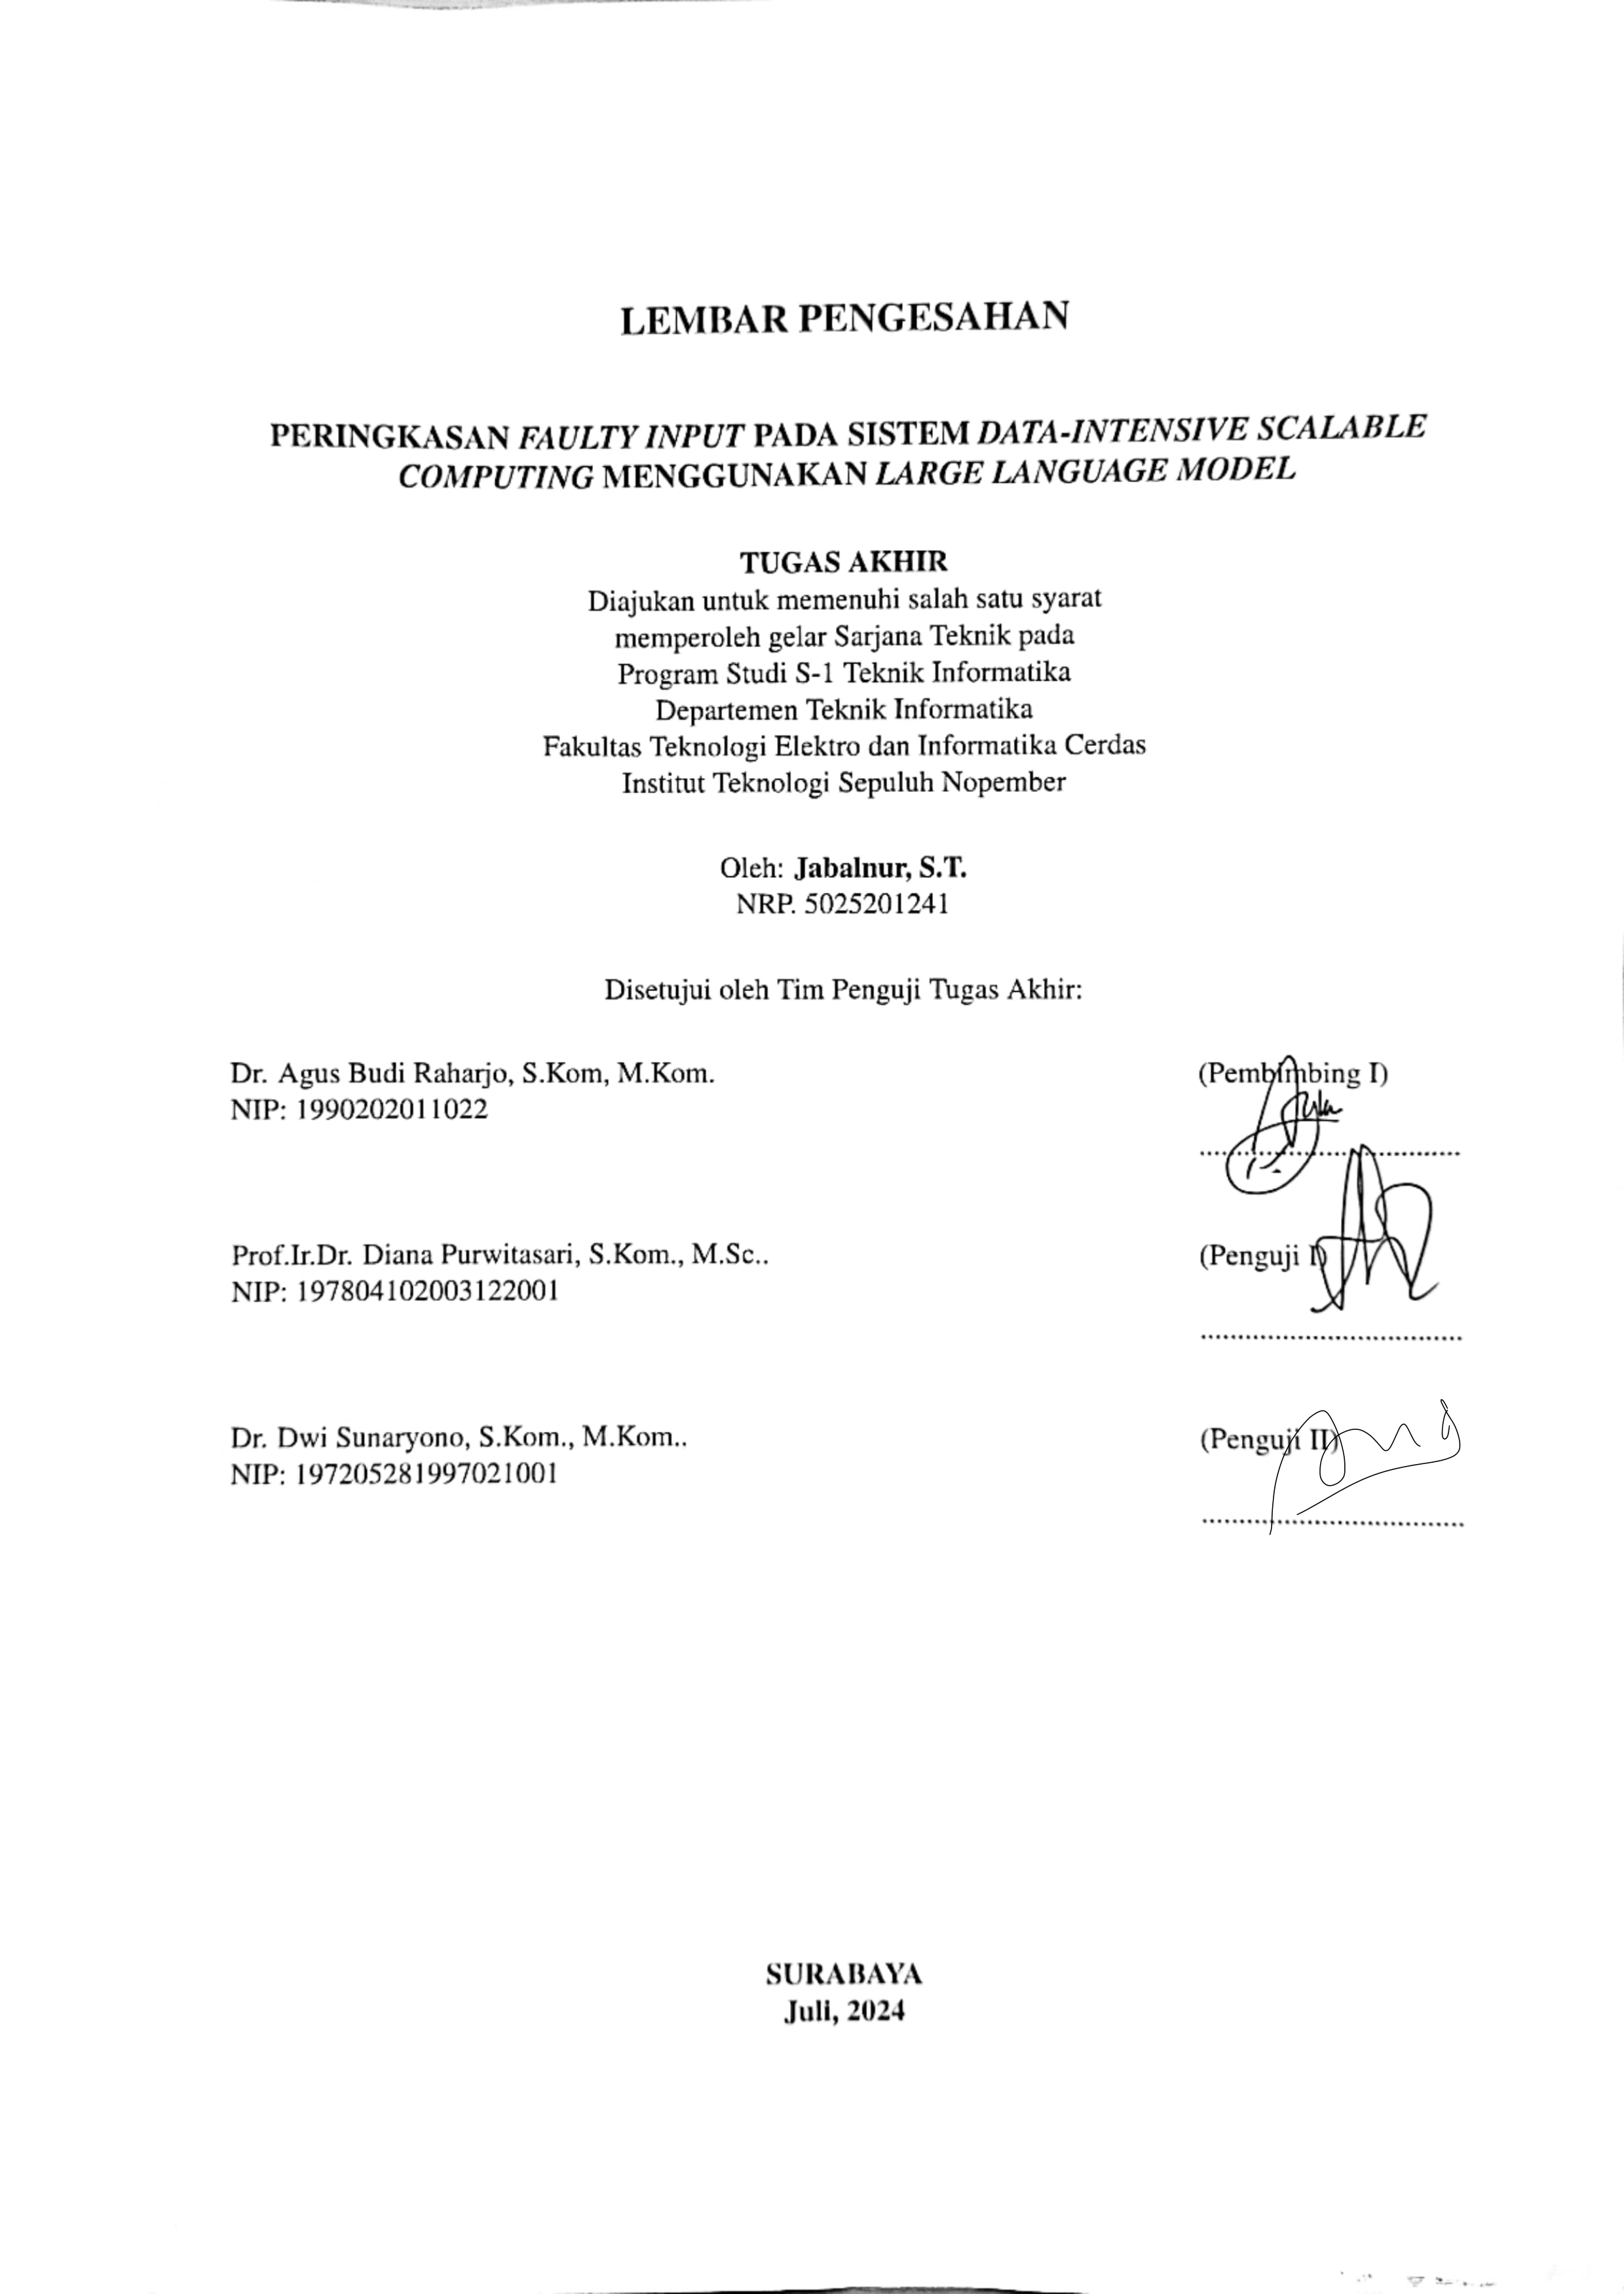
\includegraphics[width=\paperwidth, height=\paperheight]{gambar/LembarPengesahanIndo.png}
  };
\end{tikzpicture}

\cleardoublepage
\begin{center}
  \large
  \textbf{APPROVAL SHEET}
\end{center}

% Menyembunyikan nomor halaman
\thispagestyle{empty}

\begin{center}
  \textbf{\engtatitle{}}
\end{center}

\begingroup
% Pemilihan font ukuran small
\small

\begin{center}
  \textbf{FINAL PROJECT}
  \\Submitted to fulfill one of the requirements \\
  for obtaining a degree Bachelor of Engineering at \\
  Undergraduate Study Program of \engstudyprogram{} \\
  Department of \engdepartment{} \\
  Faculty of \engfaculty{} \\
  Sepuluh Nopember Institute of Technology
\end{center}

\begin{center}
  By: \textbf{\name{}}
  \\NRP. \nrp{}
\end{center}

\begin{center}
  Approved by Final Project Examiner Team:
\end{center}

\begingroup
% Menghilangkan padding
\setlength{\tabcolsep}{0pt}

\noindent
\begin{tabularx}{\textwidth}{X l}
  \advisor{}               & (Advisor I)                         \\
  NIP: \advisornip{}       &                                     \\
                           & ................................... \\
                           &                                     \\
                           &                                     \\
  \coadvisor{}             & (Co-Advisor II)                     \\
  NIP: \coadvisornip{}     &                                     \\
                           & ................................... \\
                           &                                     \\
                           &                                     \\
  \examinerone{}.          & (Examiner I)                        \\
  NIP: \examineronenip{}   &                                     \\
                           & ................................... \\
                           &                                     \\
                           &                                     \\
  \examinertwo{}.          & (Examiner II)                       \\
  NIP: \examinertwonip{}   &                                     \\
                           & ................................... \\
                           &                                     \\
                           &                                     \\
  \examinerthree{}.        & (Examiner III)                      \\
  NIP: \examinerthreenip{} &                                     \\
                           & ................................... \\
\end{tabularx}
\endgroup


\begin{center}
  Acknowledged, \\
  Head of \engdepartment{} Department \engfacultyshort{} - ITS \\

  \vspace{8ex}

  \underline{\headofdepartment{}.} \\
  NIP. \headofdepartmentnip{}
\end{center}

\begin{center}
  \textbf{\MakeUppercase{\place{}}\\\ENGMONTH{}, \the\year{}}
\end{center}
\endgroup

\cleardoublepage

% Pernyataan keaslian
\chapter*{PERNYATAAN ORISINALITAS}
\addcontentsline{toc}{chapter}{PERNYATAAN ORISINALITAS}

% Menyembunyikan nomor halaman
\thispagestyle{empty}

\vspace{2ex}

% Ubah paragraf-paragraf berikut sesuai dengan yang ingin diisi pada pernyataan keaslian

\noindent Yang bertanda tangan dibawah ini:

\noindent\begin{tabularx}{\textwidth}{l l X}
                         &   &                            \\
  Nama Mahasiswa / NRP   & : & \name{} / \nrp{}           \\
  Departemen             & : & \department{}              \\
  Dosen Pembimbing / NIP & : & \advisor{} / \advisornip{} \\
                         &   &                            \\
\end{tabularx}

Dengan ini menyatakan bahwa Tugas Akhir dengan judul "\tatitle{}" adalah hasil karya sendiri, berfsifat orisinal, dan ditulis dengan mengikuti kaidah penulisan ilmiah.

Bilamana di kemudian hari ditemukan ketidaksesuaian dengan pernyataan ini, maka saya bersedia menerima sanksi sesuai dengan ketentuan yang berlaku di Institut Teknologi Sepuluh Nopember.

\vspace{8ex}

\noindent\begin{tabularx}{\textwidth}{X l}
                     & \place{}, \ENGMONTH{} \the\year{} \\
                     &                                   \\
  Mengetahui         &                                   \\
  Dosen Pembimbing   & Mahasiswa                         \\
                     &                                   \\
                     &                                   \\
                     &                                   \\
                     &                                   \\
                     &                                   \\
  \advisor{}         & \name{}                           \\
  NIP. \advisornip{} & NRP. \nrp{}                       \\
\end{tabularx}

\cleardoublepage
\begin{center}
  \large
  \textbf{STATEMENT OF ORIGINALITY}
\end{center}

% Menyembunyikan nomor halaman
\thispagestyle{empty}

\vspace{2ex}

% Ubah paragraf-paragraf berikut sesuai dengan yang ingin diisi pada pernyataan keaslian

\noindent The undersigned below:

\noindent\begin{tabularx}{\textwidth}{l l X}
                        &   &                            \\
  Name of student / NRP & : & \name{} / \nrp{}           \\
  Department            & : & \engdepartment{}           \\
  Advisor / NIP         & : & \advisor{} / \advisornip{} \\
                        &   &                            \\
\end{tabularx}

Hereby declared that the Final Project with the title of "\engtatitle{}" is the result of my own work, is original, and is written by following the rules of scientific writing.

If in future there is a discrepancy with this statement, then I am willing to accept sanctions in accordance with provisions that apply at Sepuluh Nopember Institute of Technology.

\vspace{8ex}

\noindent\begin{tabularx}{\textwidth}{X l}
                     & \place{}, \ENGMONTH{} \the\year{} \\
                     &                                   \\
  Acknowledged       &                                   \\
  Advisor            & Student                           \\
                     &                                   \\
                     &                                   \\
                     &                                   \\
                     &                                   \\
                     &                                   \\
  \advisor{}         & \name{}                           \\
  NIP. \advisornip{} & NRP. \nrp{}                       \\
\end{tabularx}

\begin{tikzpicture}[remember picture, overlay]
  \node[anchor=north west, inner sep=0] at (current page.north west) {
      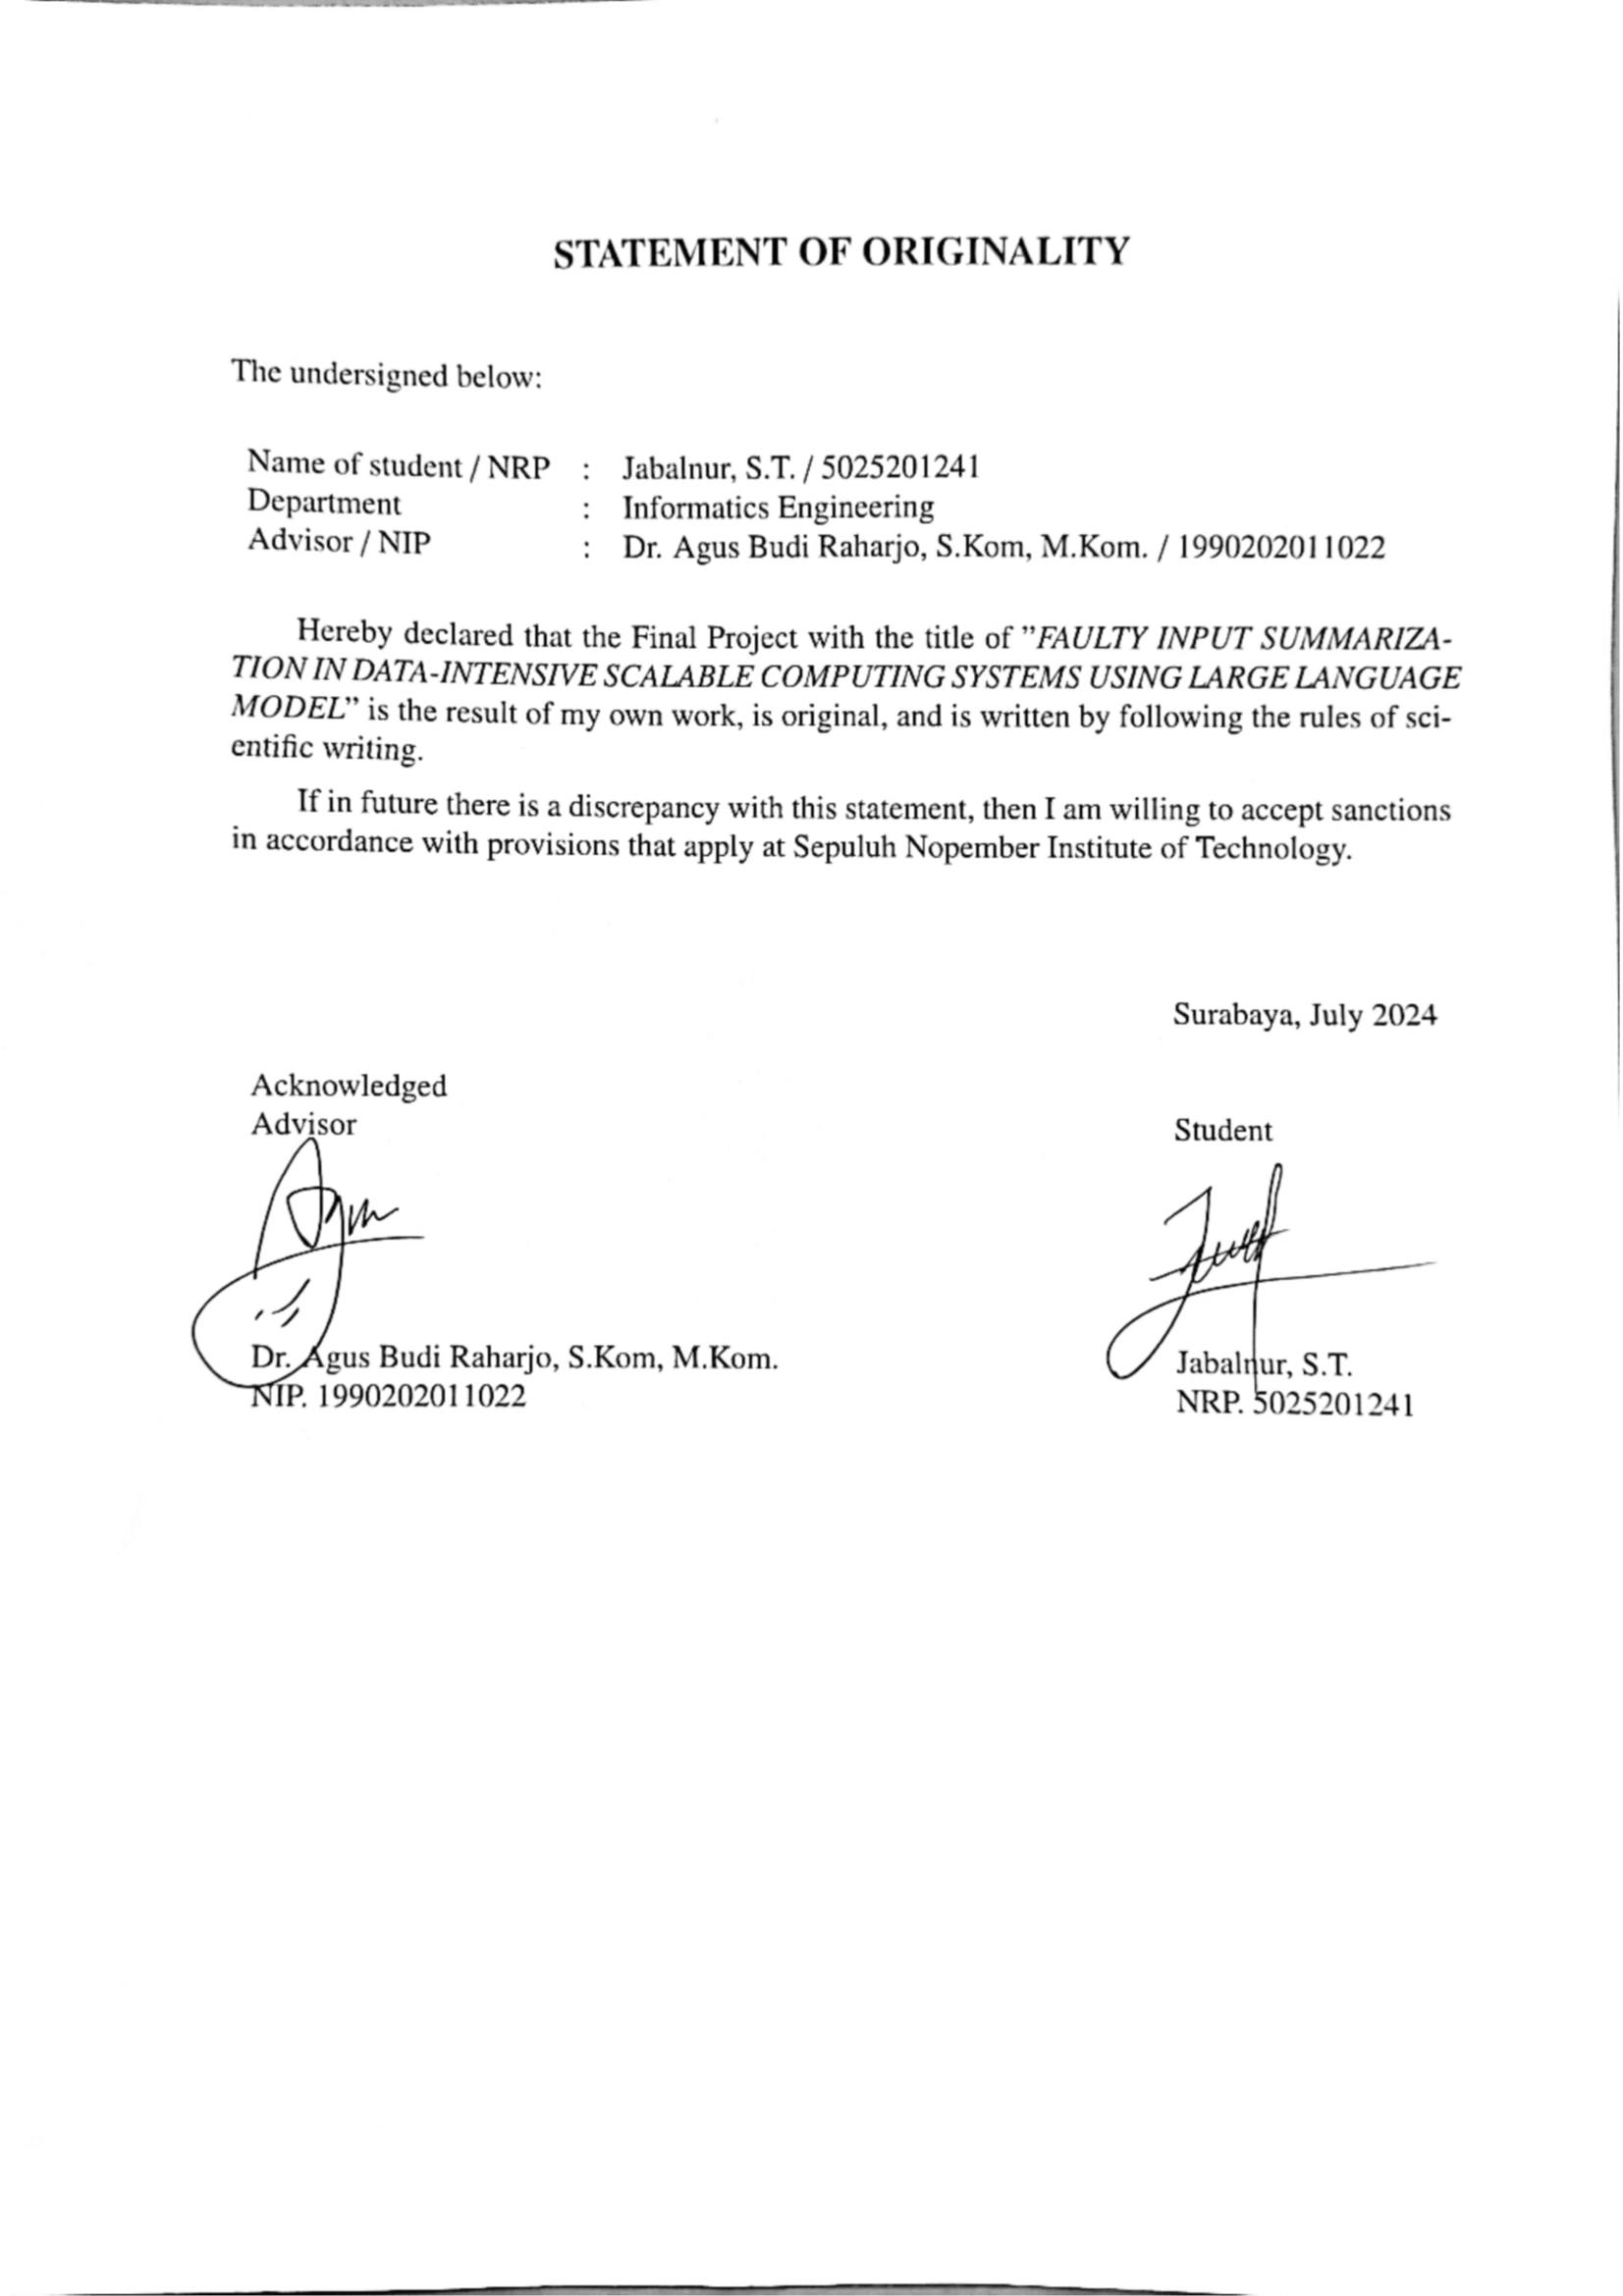
\includegraphics[width=\paperwidth, height=\paperheight]{gambar/PernyataanOrisinalitasEng.png}
  };
\end{tikzpicture}
\cleardoublepage

% Abstrak Bahasa Indonesia
\chapter*{ABSTRAK}
\addcontentsline{toc}{chapter}{ABSTRAK}

\vspace{2ex}

\begingroup
% Menghilangkan padding
\setlength{\tabcolsep}{0pt}

\noindent
\begin{tabularx}{\textwidth}{l >{\centering}m{2em} X}
  Nama Mahasiswa    & : & \name{}         \\

  Judul Tugas Akhir & : & \tatitle{}      \\

  Pembimbing        & : & 1. \advisor{}   \\
\end{tabularx}
\endgroup

% Ubah paragraf berikut dengan abstrak dari tugas akhir
% Framework pemrosesan data skala besar seperti \textit{Apache Spark} telah memungkinkan \textit{developer} untuk memproses petabyte data dengan aplikasi \textit{Data-Intensive Scalable Computing (DISC)}. Seperti halnya perangkat lunak lainnya, kesalahan dalam aplikasi \textit{DISC} adalah hal yang umum. Kesalahan tersebut dapat timbul karena dataset input yang tidak bersih atau implementasi aplikasi, yang membuat \textit{developer} harus mengidentifikasi akar penyebab di antara miliaran data input. Proses \textit{Data Provenance} dan \textit{debugging} otomatis memerlukan instrumentasi aplikasi \textit{DISC} atau melakukan \textit{search-based fault isolation} yang memakan banyak sumber daya.

% Penelitian ini bertujuan untuk menunjukkan potensi penggunaan \textit{language model} untuk menghasilkan dataset input minimal namun dapat mereproduksi kesalahan yang sama seperti yang diamati pada data masukan skala besar aslinya. Kami membuat \textit{FISUM} (\textit{Fault-inducing Inputs Summarization}), yang melatih model dengan \textit{faulty input} secara historis untuk menghasilkan baris salah baru yang minimal. \textit{FISUM} menggunakan \textit{Data Provenance Engine} yang dibangun untuk \textit{Apache Spark}, untuk memulihkan input yang menyebabkan kesalahan. Kemudian melatih sebuah \textit{lightweight language model}, \textit{DistilGPT}, menggunakan input yang menyebabkan kegagalan ini untuk menghasilkan input minimal yang mengungkapkan kesalahan yang sama.

% Pada percobaan dengan aplikasi \textit{DISC} bermasalah yang telah ada, bahkan dengan model ringan, \textit{FISUM} secara efektif dapat merangkum input yang menyebabkan kesalahan, mengurangi input asli dari alat \textit{data provenance} sebesar 99\%, namun masih dapat menyebabkan kesalahan yang sama. \textit{FISUM} menghasilkan \textit{faulty input} dalam waktu kurang dari 50 milidetik per baris, rata-rata.

Framework pemrosesan data skala besar seperti Apache Spark telah memungkinkan \textit{developer} untuk memproses petabyte data dengan aplikasi \textit{Data-Intensive Scalable Computing (DISC)}. Seperti halnya perangkat lunak lainnya, kesalahan dalam aplikasi DISC adalah hal yang umum. Kesalahan tersebut dapat timbul karena dataset input yang tidak bersih atau implementasi aplikasi, yang membuat \textit{developer} harus mengidentifikasi akar penyebab di antara miliaran data input. Proses \textit{Data Provenance} dan \textit{debugging} otomatis memerlukan instrumentasi aplikasi DISC atau melakukan \textit{search-based fault isolation} yang memakan banyak sumber daya. Penelitian ini bertujuan untuk menunjukkan potensi penggunaan \textit{language model} untuk menghasilkan dataset input minimal namun dapat mereproduksi kesalahan yang sama seperti yang diamati pada data masukan skala besar aslinya. Kami membuat FISUM (\textit{Fault-inducing Inputs Summarization}), yang melatih model dengan \textit{faulty input} secara historis untuk menghasilkan baris salah baru yang minimal dan memiliki karakteristik yang sama dengan data aslinya.

FISUM menggunakan Titian, sebuah \textit{Data Provenance Engine} yang dibangun untuk Apache Spark, untuk memulihkan input yang menyebabkan kesalahan. \textit{Data Provenance Engine} merupakan sebuah sistem yang melacak asal-usul, sejarah, dan perjalanan data dalam sebuah sistem komputasi untuk memudahkan dalam mengidentifikasi sumber kesalahan dan memahami transformasi data dari sumber aslinya hingga ke bentuk akhirnya. Titian kemudian ditanamkan ke dalam aplikasi DISC yang memiliki keluaran bermasalah untuk menemukan \textit{Faulty Input}, yaitu baris data pada dataset yang menjadi penyebab keluaran bermasalah pada aplikasi DISC. Sebuah \textit{lightweight language model}, DistilGPT2 milik HuggingFace \textit{Faulty Input} kemudian dilatih menggunakan dataset awal milik aplikasi DISC untuk membiasakan model tersebut dengan dataset aplikasi, kemudian model tersebut dilatih kembali dengan menggunakan \textit{Faulty Input} dari Titian untuk memahami karakteristik dari \textit{Faulty Input} tersebut. DistilGPT2 yang telah dilatih akhirnya dapat digunakan untuk menghasilkan \textit{Faulty Input} baru yang memiliki ukuran yang jauh lebih kecil dari ukuran aslinya dengan tetap mempertahankan kemiripan karakteristik kesalahan pada \textit{Faulty Input} awal dalam waktu yang cukup singkat.

Percobaan dilakukan dengan menguji 16 \textit{Benchmark Application} yang merupakan aplikasi DISC dengan menghitung tingkat akurasi FISUM dalam menemukan \textit{Faulty Input} pada dataset aplikasi, menghitung tingkat akurasi dari kesalahan yang dimiliki oleh \textit{Faulty Input} baru dan menghitung \textit{Mean Square Error (MSE)} dari karakteristik yang dimiliki oleh \textit{Faulty Input} awal dan baru. FISUM secara efektif dapat menemukan \textit{Faulty Input} pada aplikasi DISC dengan akurasi 100\%, dapat merangkum \textit{Faulty Input} dengan tingkat akurasi 99.4\% dalam waktu kurang dari 0.082 detik per baris, dan dapat menyajikan kemiripan karakteristik dari \textit{Faulty Input} awal dan baru dengan MSE sebesar 0.262.


% Ubah kata-kata berikut dengan kata kunci dari tugas akhir
Kata Kunci: \emph{Debugging}, \emph{Generative AI}, \emph{Faults}, \emph{Language Models}.

\cleardoublepage

% Abstrak Bahasa Inggris
\begin{center}
  \large\textbf{ABSTRACT}
\end{center}

\vspace{2ex}

\begingroup
% Menghilangkan padding
\setlength{\tabcolsep}{0pt}

\noindent
\begin{tabularx}{\textwidth}{l >{\centering}m{3em} X}
  \emph{Name}     & : & \name{}         \\

  \emph{Title}    & : & \engtatitle{}   \\

  \emph{Advisor}    & : & \advisor{}   \\

  \\
\end{tabularx}
\endgroup

% Ubah paragraf berikut dengan abstrak dari tugas akhir dalam Bahasa Inggris
\emph{Large-scale data processing frameworks like Apache Spark have enabled developers to process petabytes of data with Data-Intensive Scalable Computing (DISC) applications. Like any other software, faults in DISC applications are common. These faults can arise due to unclean input datasets or application implementation, requiring developers to identify the root cause among billions of input data. The process of Data Provenance and automated debugging requires instrumenting DISC applications or performing search-based fault isolation, which consumes significant resources.}

\emph{This study aims to demonstrate the potential use of language models to generate minimal input datasets capable of reproducing the same faults observed in the original large-scale input data. We introduce FISUM (Fault-inducing Inputs Summarization), which trains a model on historically faulty inputs to generate new minimal faulty rows. FISUM leverages the Data Provenance Engine built for Apache Spark to recover fault-inducing inputs. It then trains a lightweight language model, DistilGPT, on these failure-inducing inputs to generate minimal fault-revealing inputs.}

\emph{In experiments with existing faulty DISC applications, even with a lightweight model, FISUM effectively summarizes fault-inducing input, reducing the original input from the data provenance tool by 99\%, while still inducing the same fault. FISUM generates faulty inputs in under 50 milliseconds per row, on average.}

% Ubah kata-kata berikut dengan kata kunci dari tugas akhir dalam Bahasa Inggris
\emph{Keywords}: \emph{Debugging}, \emph{Generative AI}, \emph{Faults}, \emph{Language Models}.

\cleardoublepage

% Kata pengantar
\chapter*{KATA PENGANTAR}
\addcontentsline{toc}{chapter}{KATA PENGANTAR}

\vspace{2ex}

% Ubah paragraf-paragraf berikut dengan isi dari kata pengantar

Puji dan syukur penulis panjat kan kepada Tuhan yang Maha Esa atas
berkat, rahmat, dan karunia-Nya sehingga tugas akhir yang berjudul "\tatitle" dapat
diselesaikan dengan baik sebagai salah satu syarat dalam menyelesaikan Strata-1
pada Departemen \studyprogram{}, \faculty{}, \institute{}.

Penulis menyadari bahwa dalam penyusunan dan penulisan tugas akhir ini
tidak lepas dari bantuan, bimbingan, serta dukungan dari berbagai pihak, dari masa
perkuliahan hingga penyusunan tugas akhir. Oleh karena itu, penulis menyampaikan
terima kasih kepada:

\begin{enumerate}[nolistsep, noitemsep,topsep=0pt]

  \item Kedua orang tua penulis, Bapak Jamaluddin S, S.Pd., dan 
  Ibu Hj. Nurbaya Nur yang tidak pernah lelah dalam mendidik dan 
  memberikan dukungan, doa, serta semangat kepada penulis.

  \item Bapak \advisor{}, selaku Dosen Pembimbing I Tugas 
  Akhir penulis yang senantiasa membimbing
  dan menyediakan waktu, tenaga, dan perhatiannya di sepanjang 
  pengerjaan tugas akhir ini.

  \item Bapak Ali Gulzar, Ahmad, dan Gista yang telah memberikan
  bimbingan, arahan, bantuin selama pengerjaan tugas akhir ini.

  \item Bapak dan Ibu dari Direktorat Jenderal Pendidikan Tinggi
  Kementerian Pendidikan, Kebudayaan, Riset, dan Teknologi yang telah
  memberikan beasiswa LPDP yang telah membantu penulis dalam menyelesaikan
  tugas akhir ini.

  \item Segenap Dosen dan Tenaga Pendidik \department{} \faculty{} \institute{}
  yang telah banyak membantu semasa perkuliahan dan dalam penyelesaian tugas akhir.

  \item Saudara-saudara \emph{Backstreet} yang telah memberikan
  bantuan, semangat, waktu, serta segala macam hal yang telah membawa
  penulis hingga bisa menjadi seperti sekarang ini.

  \item Sahabat-sahabat dari Kontrakan KP IV No.5B yang telah memberikan
  dukungan, semangat, dan bantuan dalam menjalani perkuliahan ini.

  \item Teman-teman dari Kanda ITS yang telah memberikan dukungan, semangat,
  dan bantuan selama masa perkuliahan dan pengerjaan tugas akhir.

  \item Seluruh pihak yang tidak sempat tersebutkan dan tanpa sadar telah
  menjadi inspirasi serta banyak membantu penulis dalam menyelesaikan tugas akhir.

\end{enumerate}

Akhir kata, penulis menyadari bahwa tugas akhir ini mash jauh dari kata
sempurna, oleh karenanya diharapkan segala bentuk saran serta masukan yang
membangun dari berbagai pihak. Semoga tugas akhir ini dapat memberikan
sumbangsih dan manfaat besar bagi kehidupan manusia

\begin{flushright}
  \begin{tabular}[b]{c}
    \place{}, \MONTH{} \the\year{} \\
    \\
    \\
    \\
    \\
    \name{}
  \end{tabular}
\end{flushright}

\cleardoublepage

% Daftar isi
\renewcommand*\contentsname{DAFTAR ISI}
\label{chap:daftar isi}
\addcontentsline{toc}{chapter}{\contentsname}
\tableofcontents
\cleardoublepage



% Daftar gambar
\renewcommand*\listfigurename{DAFTAR GAMBAR}
\label{chap:daftar gambar}
\addcontentsline{toc}{chapter}{\listfigurename}
\listoffigures
\cleardoublepage

% Daftar tabel
\renewcommand*\listtablename{DAFTAR TABEL}
\label{chap:daftar tabel}
\addcontentsline{toc}{chapter}{\listtablename}
\listoftables
\cleardoublepage

% Daftar kode
\renewcommand*\lstlistlistingname{DAFTAR KODE}
\label{chap:daftar kode}
\addcontentsline{toc}{chapter}{\lstlistlistingname}
\lstlistoflistings
\cleardoublepage

% Nomor halaman isi dimulai dari sini
\pagenumbering{arabic}

% Bab 1 pendahuluan
\chapter{PENDAHULUAN}\label{chap:pendahuluan}

% Ubah bagian-bagian berikut dengan isi dari pendahuluan

\section{Latar Belakang}\label{sec:latarbelakang}

Analisis data modern memerlukan penanganan data berskala 
terabyte yang tersebar di berbagai mesin. Untuk membuat 
ini dapat dilakukan, kerangka kerja 
\emph{Data Intensive Scalable Computing (DISC)} seperti 
Apache Spark~\cite{zaharia2010,spark} dan 
Google MapReduce~\cite{dean2008} memungkinkan analis 
data untuk membuat aplikasi terdistribusi. Volume besar 
data input untuk aplikasi DISC, ditambah dengan sifat 
terdistribusi dari program, membuat debugging menjadi 
sangat menantang.
Bayangkan sebuah program yang menghitung rata-rata 
curah hujan per tahun di Amerika Serikat. Ini 
memerlukan penghitungan rata-rata dari puluhan 
juta nilai yang dikumpulkan dari sensor yang 
tersebar di seluruh negeri. Setelah menjalankan 
program, analis memperhatikan bahwa nilai rata-rata 
yang dihasilkan sangat tinggi dan mencurigakan. 
Bagaimana programmer akan mendiagnosis penyebab 
kesalahan ini?

Beberapa penelitian dalam debugging program telah 
berfokus pada pengurangan ukuran input yang 
menyebabkan kesalahan~\cite{zeller2002,misherghi2006,kirschner2020,clause2009}.
Banyak dari teknik ini 
adalah varian dari algoritma delta debugging, 
yang bekerja dengan menjalankan program berulang 
kali dengan segmen-segmen berbeda dari input yang 
menyebabkan kesalahan hingga algoritma tersebut 
menemukan ukuran input minimal. Teknik pengurangan 
input tradisional ini, meskipun telah dicoba~\cite{gulzar2018}, tidak 
dapat diterapkan pada aplikasi DISC karena memerlukan 
eksekusi berulang yang lambat dan memakan banyak 
sumber daya.

Dalam penelitian ini, kami mengusulkan teknik berbasis 
\emph{large language model} (LLM) yang efisien untuk 
merangkum data yang bermasalah, yang mungkin mencakup 
jutaan baris, menjadi hanya beberapa baris yang tetap 
dapat mereproduksi kesalahan. Kami mewujudkan ide ini 
dalam alat yang disebut FISUM, sebuah sistem 
\emph{Fault-inducing Inputs Summarization}. 
Inti dari teknik kami adalah bahwa LLM generatif 
modern dapat dilatih untuk menangkap pola input 
yang memicu kesalahan dari data besar. Hasil dari 
pelatihan model ini kemudian dapat digunakan untuk 
menghasilkan input baru yang menyebabkan pola 
kesalahan yang sama.

Teknik kami memerlukan proses \emph{pre-training} 
dari model GPT versi ringan, distilGPT, pada seluruh 
data input. Langkah \emph{unsupervised} ini 
memungkinkan model untuk mempelajari struktur 
dasar dan pola dari data tersebut. Kami kemudian 
menggunakan Titian~\cite{interlandi2015} untuk mengambil subset besar 
dari input yang dianggap mencurigakan terkait 
dengan eksekusi yang salah. distilGPT kemudian 
dilatih ulang pada data mencurigakan ini untuk 
membiasakannya dalam menghasilkan input yang 
menyebabkan kesalahan. Akhirnya, distilGPT diarahkan 
untuk menghasilkan data yang dapat mereproduksi 
kesalahan tersebut.
Untuk mengevaluasi teknik kami, kami menggunakan satu 
set program \emph{benchmark} dari penelitian sebelumnya 
tentang \emph{debugging} dan pengujian aplikasi 
DISC~\cite{gulzar2019,humayun2023,zhang2021}. 

\section{Rumusan Permasalahan}
\label{sec:permasalahan}

Berdasarkan latar belakang di atas, maka dapat ditarik rumusan masalah sebagai berikut:

\begin{enumerate}[nolistsep]

   \item Apakah input yang bermasalah yang dihasilkan oleh FISUM masih mempertahankan kemampuan deteksi kesalahan?

   \item Berapa banyak persentase pengurangan input bermasalah yang dapat dihasilkan oleh FISUM dari dataset yang diberikan?

   \item Berapa lama waktu yang dibutuhkan untuk menghasilkan input bermasalah oleh FISUM?
   
   \item Berapa lama waktu yang dibutuhkan untuk melatih tiap model dengan FISUM?

\end{enumerate}

\section{Batasan Masalah}
\label{sec:batasanmasalah}

Batasan masalah penelitian ini adalah sebagai berikut:

\begin{enumerate}[nolistsep]

  \item Implementasi algoritma menggunakan bahasa Python dan Scala.

  \item Pembuatan sistem hanya berfokus pada proses \emph{debugging} dan \emph{generate new faulty input} bukan pada aplikasi DISC yang test inputnya akan didebug.

  \item Proses \emph{debugging} dan \emph{generate new faulty input} hanya berfokus pada 16 \emph{benchmark program} yang berjalan di aplikasi DISC. 

  \item Test input berupa \emph{text} yang menyatukan beberapa kolom yang dibutuhkan

\end{enumerate}

\section{Tujuan}
\label{sec:Tujuan}

Tujuan penelitian ini adalah sebagai berikut:

\begin{enumerate}[nolistsep]

  \item Mengevaluasi kemampuan deteksi kesalahan dari input bermasalah yang dihasilkan oleh FISUM.
  \item Mengukur persentase pengurangan input bermasalah yang dihasilkan oleh FISUM dari dataset yang diberikan.
  \item Mengukur waktu yang dibutuhkan untuk menghasilkan input bermasalah oleh FISUM.
  \item Mengukur waktu yang dibutuhkan untuk melatih tiap model dengan FISUM.

\end{enumerate}

\section{Manfaat}
\label{sec:Manfaat}

Manfaat penelitian ini adalah sebagai berikut:

\begin{enumerate}[nolistsep]
  \item Membantu \ meningkatkan \ kualitas \  perangkat \  lunak \ yang \  berjalan \ pada \ platform \emph{Data-Intensive Scalable Computing (DISC)},\  seperti \ Apache \ Hadoop, \ Apache Spark, dan Apache Flink.
  \item Membantu menghemat waktu dan upaya yang diperlukan untuk mengidentifikasi dan mengatasi masalah dalam aplikasi DISC.
  \item Meningkatkan produktivitas pengembang perangkat lunak.
  \item Membantu penilitian yang terkait dengan aplikasi DISC.

\end{enumerate}

\cleardoublepage

% Bab 2 tinjauan pustaka
\chapter{TINJAUAN PUSTAKA}
\label{chap:tinjauanpustaka}

\section{Penelitian Terkait}
\label{sec:penelitianTerkait}

% Contoh input gambar
\begin{figure}[H]
  \centering

  % Ubah dengan nama file gambar dan ukuran yang akan digunakan
  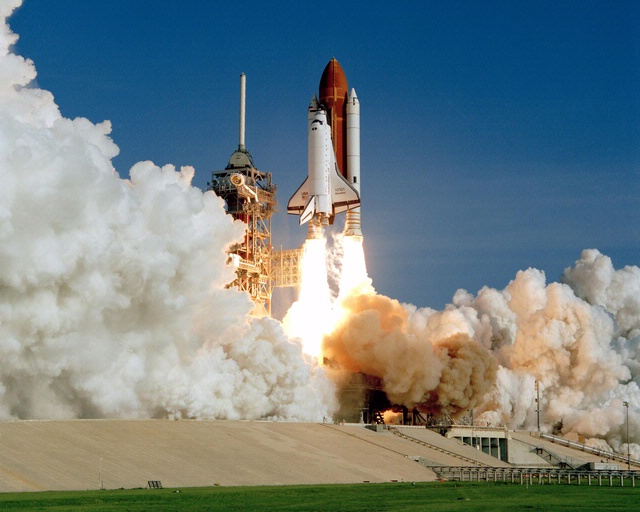
\includegraphics[scale=0.35]{gambar/roketluarangkasa.jpg}

  % Ubah dengan keterangan gambar yang diinginkan
  \caption{Diagram \emph{Fishbone}}
  \label{fig:fishbone}
\end{figure}

\subsection{\emph{Automated Debugging in Data-Intensive Scalable Computing}}
\label{subsec:Automated Debugging in Data-Intensive Scalable Computing}

Penelitian yang dilakukan oleh Muhammad Ali Gulzar dan rekan-rekannya fokus pada pengembangan beban kerja \emph{Big Data Analytics}. Mereka menghadapi tantangan dalam \emph{debugging}, terutama terkait dengan data tidak terstruktur dan asumsi yang salah mengenai data, yang sering menyebabkan kesalahan dalam program. Untuk mengatasi masalah ini, penelitian ini memperkenalkan metode baru yang disebut BIGSIFT, yang berfokus pada menemukan lokasi data yang menyebabkan kegagalan. Metode yang digunakan yaitu menggabungkan isolasi kesalahan otomatis dalam rekayasa perangkat lunak dengan \emph{provenans} data dalam sistem basis data. Hasil dari penelitian ini adalah peningkatan drastis dalam akurasi dalam menentukan lokasi kesalahan, dengan hasil yang lebih akurat hingga ribuan hingga jutaan kali lipat dibandingkan dengan metode sebelumnya seperti provenans data Titian dan \emph{Delta Debugging}. Dengan demikian, penelitian ini berpotensi memberikan manfaat besar dalam mempercepat proses \emph{debugging} pada beban kerja \emph{Big Data Analytics}, sehingga pengembang dapat mengidentifikasi dan memperbaiki masalah lebih efisien.

\subsection{\emph{BigFuzz: Efficient Fuzz Testing for Data Analytics Using Framework Abstraction}}
\label{subsec:BigFuzz: Efficient Fuzz Testing for Data Analytics Using Framework Abstraction}

Dalam penelitian yang dilakukan oleh Qian Zhang dan timnya, mereka mengatasi tantangan dalam pengujian otomatis untuk sistem data-intensive scalable computing (DISC), yang sangat penting untuk menangani kumpulan data besar dalam konteks analisis big data. Masalah utamanya terletak pada kompleksitas intrinsik dari aplikasi berbasis data semacam itu, di mana data seringkali tidak lengkap, terus berubah, dan sulit untuk diprediksi. Pengujian \emph{fuzzing} tradisional, meskipun efektif di domain lain seperti keamanan, menghadapi hambatan yang signifikan ketika diterapkan langsung pada analisis big data. Alasannya termasuk lamanya latensi sistem DISC, tidak praktisnya cakupan cabang konvensional, dan kesulitan dalam menghasilkan data yang bermakna dengan mutasi acak. Untuk mengatasi tantangan ini, para peneliti mengusulkan alat pengujian \emph{fuzzing} yang dipandu cakupan yang baru untuk analisis big data, yang disebut BigFuzz. Alat ini berfokus pada pengujian logika aplikasi daripada peningkatan cakupan kode kerangka kerja, dengan mengabstraksi kerangka kerja DISC menggunakan spesifikasi. BigFuzz juga menggunakan operator \emph{schema-aware data mutation} berdasarkan analisis mendalam tentang jenis kesalahan aplikasi DISC. Hasil penelitian menunjukkan bahwa BigFuzz secara signifikan mempercepat proses \emph{fuzzing}, meningkatkan cakupan kode, dan meningkatkan deteksi kesalahan dalam aplikasi DISC, menjadikannya alat berharga untuk \emph{debugging} beban kerja analisis \emph{big data}, dapat diterapkan pada beragam program, dan mampu menemukan lebih banyak kesalahan dibandingkan dengan pendekatan terkini yang menggunakan eksekusi simbolik.

\subsection{\emph{BigTest: A Symbolic Execution Based Systematic Test Generation Tool for Apache Spark}}
\label{subsec:BigTest: A Symbolic Execution Based Systematic Test Generation Tool for Apache Spark}

Muhammad Ali Gulzar dan timnya melakukan penelitian dalam bidang sistem komputasi berbasis data yang besar (DISC), seperti MapReduce milik Google, Apache Hadoop, dan Apache Spark, yang digunakan luas dalam layanan produksi. Meskipun aplikasi DISC sangat populer, seringkali kualitas aplikasinya kurang baik karena kurangnya pengujian yang menyeluruh dan otomatis. Saat ini, pengujian aplikasi DISC biasanya hanya menggunakan contoh kecil acak dari data masukan, yang mungkin tidak cukup untuk menemukan masalah dalam program. Pengujian aplikasi DISC memiliki tantangan tersendiri karena menggabungkan operasi aliran data dan relasional, serta fungsi yang bisa sangat kompleks.Untuk mengatasi masalah ini, para peneliti memperkenalkan kerangka pengujian putih yang baru bernama BigTest. BigTest digunakan untuk program Apache Spark dan secara otomatis menghasilkan data buatan untuk pengujian yang efektif dan efisien. BigTest menggabungkan eksekusi simbolik fungsi pengguna dengan spesifikasi logis operasi aliran data dan relasional untuk mengeksplorasi semua jalur dalam aplikasi DISC. Hasil eksperimen menunjukkan bahwa BigTest mampu menemukan dua kali lipat lebih banyak masalah daripada menggunakan seluruh dataset dengan waktu pengujian yang jauh lebih singkat (194 kali lebih cepat). BigTest diimplementasikan sebagai alat baris perintah berbasis Java dengan file biner pra-kompilasi. Pengguna dapat menyesuaikan preferensi melalui file konfigurasi, termasuk program target, batasan eksplorasi \emph{loop}, dan pemilihan penyelesaian teorema. Penelitian ini berpotensi meningkatkan pengujian aplikasi DISC, sehingga masalah dalam program dapat ditemukan dengan lebih efektif dan efisien.

\subsection{\emph{Titian: Data Provenance Support in Spark}}
\label{subsec:Titian: Data Provenance Support in Spark}

Matteo Itterlandi dan timnya mengatasi tantangan yang sulit dalam melakukan \emph{debugging} pada logika pemrosesan data di dalam sistem Data-Intensive Scalable Computing (DISC). Biasanya, \emph{debugging} dalam sistem ini memakan banyak waktu dan usaha karena kurangnya alat \emph{debugging} yang memadai, seringkali memerlukan pengumpulan bukti secara manual dari file log dan mencoba-coba. Untuk mempermudah proses ini, mereka mengembangkan Titian, sebuah perpustakaan yang memungkinkan pelacakan asal data - mengikuti jejak data melalui berbagai transformasi di Apache Spark. Dengan menggunakan ekstensi Spark Titian, ilmuwan data dapat dengan cepat mengidentifikasi data masukan yang menjadi penyebab potensial kesalahan atau hasil yang tidak biasa. Titian terintegrasi dengan baik ke dalam \emph{platform} Spark dan menyediakan dukungan asal data dengan kecepatan interaktif, jauh lebih cepat dibandingkan dengan solusi yang sudah ada, dengan dampak minimal pada kinerja pekerjaan Spark. \emph{Overhead} untuk mengambil jejak data biasanya tidak lebih dari 30\% dari waktu eksekusi pekerjaan dasar. Penelitian ini secara signifikan meningkatkan efisiensi dalam \emph{debugging} logika pemrosesan data dalam sistem DISC, memberikan pendekatan yang lebih efektif dan menghemat waktu bagi ilmuwan data dalam mengidentifikasi dan memecahkan masalah.

\subsection{\emph{Automatic Romanian Text Generation Using GPT-2}}
\label{subsec:Automatic Romanian Text Generation Using GPT-2}

Marius Cristian Buzea dan timnya melakukan penelitian di bidang pemrosesan bahasa alami (NLP), khususnya dalam menghasilkan teks. Mereka menggunakan model transformer besar yang sudah dilatih sebelumnya seperti GPT-2 dan GPT-3 dari OpenAI, serta BERT dari Google. Penelitian ini mengembangkan model NLG berbasis arsitektur GPT-2 untuk menghasilkan teks dalam bahasa Rumania dengan menggunakan teks yang dianotasi secara manual. Model kecil GPT-2 Rumania, bernama MCBGPT-2, dilatih dan diuji dengan 24 ribu berita. Selain itu, model GPT-2 Rumania yang ada, RoGPT-2, juga digunakan dalam eksperimen. Evaluasi menggunakan metrik otomatis seperti BLEU, ROUGE, BLEURT, dan BERTScore menunjukkan bahwa model MCBGPT-2 dan RoGPT-2 memiliki kinerja yang serupa dalam tugas penghasil teks untuk bahasa Rumania, dengan MCBGPT-2 memerlukan lebih sedikit data untuk proses pelatihannya. Hasil eksperimen menunjukkan bahwa MCBGPT-2 dan RoGPT-2 memberikan kinerja yang hampir sama dalam menghasilkan teks dalam bahasa Rumania, namun MCBGPT-2 memerlukan lebih sedikit data selama pelatihan. Selain itu, arsitektur transformer yang digunakan oleh GPT-2 memungkinkan kecepatan pelatihan yang lebih tinggi dan kemampuan paralelisasi yang lebih baik. Penelitian ini menyimpulkan bahwa model MCBGPT-2 adalah alternatif yang efisien untuk model RoGPT-2 yang ada, terutama dalam menghasilkan kalimat panjang menggunakan data pelatihan yang lebih sedikit.

\section{Dasar Teori}
\label{sec:dasarTeori}

Pada subbab ini akan dijelaskan dasar teori yang digunakan dalam penelitian ini. Berdasarkan pada subbab 2.1, penelitian ini akan diterapkan pada sistem Data-Intensive Scalable Computing (DISC). DISC itu sendiri merupakan pendekatan komputasi yang terfokus pada pengolahan dan analisis data dalam skala besar di mana tujuan utamanya adalah memastikan bahwa data ini dapat digunakan untuk mendapatkan wawasan berharga, mendukung pengambilan keputusan, dan mengidentifikasi pola yang relevan dalam data tersebut [8]. Hingga saat ini, telah banyak platform yang dibangun untuk dapat memonitoring proses kerja sistem DISC [9].

Sistem DISC ini akan dibangun menggunakan Apache Spark, yaitu sebuah platform pemrosesan data open source yang sangat kuat dan populer. Dirancang untuk mengatasi tantangan pemrosesan data dalam skala besar, Spark menyediakan kerangka kerja yang efisien untuk mengelola dan menganalisis data dalam volume besar dengan kecepatan tinggi. Salah satu fitur utama dari Spark adalah kemampuannya untuk menggabungkan pemrosesan batch dan pemrosesan aliran data dalam satu framework yang kuat, yang memungkinkan pengguna untuk melakukan analisis data real-time dan batch dengan efisiensi tinggi. Spark juga mendukung pemrosesan data terdistribusi dan pemrosesan paralel, yang membuatnya sangat cocok untuk tugas-tugas yang membutuhkan komputasi tingkat tinggi. Ini memiliki antarmuka pemrograman yang beragam, termasuk Python, Scala, dan Java, sehingga dapat diakses oleh berbagai pengembang. Spark juga memiliki perpustakaan yang kaya, seperti MLib untuk pembelajaran mesin, SQL untuk kueri data, dan Streaming untuk pemrosesan aliran data [10]. Platform ini telah menjadi pilihan populer dalam berbagai industri, termasuk analisis data, ilmu data, dan pemrosesan aliran data [11]. 

Untuk dapat memisahkan antara data benar dan data yang bermasalah akan digunakan sebuah library bernama Spark Titian. Spark Titian merupakan sebuah perpustakaan yang dirancang untuk memungkinkan provenans data interaktif dalam lingkungan Apache Spark. Titian terintegrasi dengan antarmuka pemrograman Spark, yang berdasarkan abstraksi Resilient Distributed Dataset (RDD) yang menentukan serangkaian transformasi dan tindakan untuk memproses kumpulan data. Data yang dihasilkan dari serangkaian transformasi tertentu yang menghasilkan RDD dapat disimpan dalam memori. Spark menjaga sejarah transformasi program sehingga dapat memulihkan partisi RDD yang hilang dalam kasus kegagalan. Titian memperkaya abstraksi RDD dengan kemampuan provenans data yang sangat terinci. Ini memungkinkan seorang pemrogram Spark untuk mengakses referensi LineageRDD dari RDD tertentu, memfasilitasi fungsionalitas pelacakan data, yaitu kemampuan untuk berpindah mundur (atau maju) dalam aliran data program Spark. Dari referensi LineageRDD tertentu, yang sesuai dengan posisi dalam eksekusi program, dapat memanggil transformasi RDD asli apa pun, menghasilkan RDD baru yang memproses subset data yang dirujuk oleh LineageRDD. Kemampuan ini menyederhanakan kemampuan untuk melacak baik ke belakang maupun ke depan dalam aliran data, memungkinkan eksekusi serangkaian transformasi RDD asli baru pada data yang dirujuk. Dukungan pelacakan yang disediakan oleh LineageRDD terintegrasi dengan operator batch internal Spark dan mekanisme toleransi kesalahan. Akibatnya, Titian dapat digunakan dalam sesi terminal Spark, menyediakan dukungan provenans data interaktif bersama dengan kueri ad-hoc Spark asli [7].

Selain itu, untuk dapat mengganti data yang bermasalah dengan data yang benar, akan digunakan sebuah model yang disediakan oleh HugginFace. HuggingFace adalah sebuah perusahaan yang dikenal sebagai pemimpin dalam bidang pemrosesan bahasa alami (Natural Language Processing, NLP). Misi inti mereka adalah membuat teknologi NLP yang kuat dan canggih lebih mudah diakses oleh para peneliti, ilmuwan data, pengembang, dan perusahaan [12]. Salah satu kontribusi utama HuggingFace adalah penyediaan berbagai model NLP "state-of-the-art" yang telah dilatih dengan data besar, seperti model BERT, DistilBert, GPT-2, DistilGPT2, dan banyak lagi. Model-model ini sangat kuat dan dapat digunakan dalam berbagai tugas, seperti penerjemahan bahasa, analisis sentimen, generate teks otomatis, dan pemahaman bahasa alami [13]. Selain itu, HuggingFace juga menyediakan API yang mempermudah penggunaan model NLP tersebut. Mereka juga mengembangkan alat-alat dan perpustakaan (library) yang mendukung pengembangan dan penelitian di bidang NLP [14]. Dengan demikian, HuggingFace berperan penting dalam memperluas akses ke teknologi NLP canggih, memungkinkan inovasi di berbagai industri, termasuk pemrosesan teks, layanan pelanggan, penelitian akademik, dan banyak lagi [15].

DistilGPT2 Model dipilih sebagai model yang akan digunakan pada penelitian ini. DistilGPT2 adalah model NLP yang dikembangkan oleh HuggingFace, yang merupakan versi ringan (distil) dari model GPT-2 (Generative Pre-trained Transformer 2). Keunggulan DistilGPT2 terletak pada efisiensi komputasi, membuatnya sangat cocok untuk aplikasi yang membutuhkan pemrosesan teks cepat dalam skala besar. DistilGPT2 mempertahankan arsitektur dasar GPT-2 dengan lapisan dan parameter lebih sedikit, membuatnya lebih ringan dan cepat. Meskipun lebih kecil, DistilGPT2 mampu menghasilkan teks dengan baik dan cocok untuk aplikasi NLP pada perangkat dengan sumber daya terbatas. Hasil evaluasi menunjukkan bahwa DistilGPT2 memiliki performa yang kompetitif dan efisien. Hal ini membuat DistilGPT2 menjadi pilihan yang menarik dalam pengembangan aplikasi yang bergantung pada analisis teks dengan kecepatan dan efisiensi [6].

Untuk dapat menghubungkan antara DistilGPT2 Model dan program DISC yang menggunakan Titian, penelitian ini akan memanfaatkan FastAPI. FastAPI adalah kerangka kerja web Python yang dikenal dengan kinerja tinggi, kemudahan pengembangan, dan otomatisasi pembuatan dokumentasi API. Dibangun di atas Python 3.6+ yang mendukung asynchronous programming, FastAPI dapat menangani banyak permintaan dengan cepat. Kerangka kerja ini menggunakan teknologi seperti Starlette dan Pydantic untuk memastikan penanganan permintaan HTTP yang efisien dan validasi data yang kuat [17]. Hingga kini FastAPI telah banyak dimanfaatkan untuk keperluan machine learning dan data science dan terbukti 45% jauh lebih baik dibandingkan dengan Flask [18]. Flask adalah framework web Python yang ringan dan fleksibel yang menekankan kesederhanaan dan kemampuan untuk diperluas. Ini menyediakan fitur dasar untuk pengembangan web dan memungkinkan pengembang memilih dan mengintegrasikan ekstensi berdasarkan kebutuhan proyek mereka [19].

DistilGPT2 Model yang ditanamkan ke dalam FastAPI kemudian akan di-deploy menggunakan Amazon Web Service (AWS) EC2. AWS adalah platform komputasi awan yang dikelola oleh Amazon. AWS menyediakan berbagai layanan komputasi, penyimpanan, database, jaringan, dan lainnya yang dapat digunakan oleh perusahaan dan pengembang untuk menjalankan aplikasi mereka di lingkungan awan. Amazon EC2 adalah salah satu layanan inti di AWS yang memungkinkan pengguna untuk menyewa mesin virtual (instance) di cloud. Pengguna dapat memilih berbagai jenis instance yang sesuai dengan kebutuhan mereka, seperti instance berkinerja tinggi, instance berbasis GPU, atau instance berbiaya rendah. AWS EC2 memungkinkan pengguna untuk dengan cepat meluncurkan, mengelola, dan menghentikan instance sesuai kebutuhan, sehingga mereka dapat mengskalakan aplikasi mereka sesuai dengan permintaan dan menghemat biaya saat instance tidak digunakan [20]. Dibandingkan dengan kompetitornya, AWS EC2 menawarkan solusi yang lebih baik di mana pengguna dapat memiliki kesempatan untuk memilih fitur yang diinginkan sesuai kebutuhan [21]. 

Pengembangan sistem akan menggunakan 2 bahasa pemrograman. Pada proses training awal model dan pembuatan FastAPI, bahasa pemrograman yang akan digunakan adalah Python. Sedangkan pada pembuatan sistem yang akan mengonsumsi FastAPI, bahasa pemrograman yang akan digunakan adalah Scala. Python dipilih untuk proses training awal model dan pembuatan FastAPI karena memiliki sintaksis yang mudah dipahami, ekosistem yang kaya, serta banyak library dan framework yang mendukung pengembangan aplikasi machine learning dan web termasuk HuggingFace. Kelebihan Python dalam kesederhanaan dan kemudahan penggunaan membuatnya menjadi pilihan utama dalam fase awal pengembangan [22]. Sementara itu, Scala dipilih untuk pembuatan sistem yang mengonsumsi FastAPI karena Scala menawarkan keunggulan dalam hal konkurensi dan eksekusi paralel, yang dapat meningkatkan kinerja sistem secara signifikan. Pemilihan Scala juga didorong oleh keandalan dan ekosistem yang mapan, terutama dalam pengembangan aplikasi berukuran besar [23]. Dibandingkan dengan Java pada bidang Natural Language Processing (NLP), Scala dianggap lebih unggul karena ekosistemnya yang lebih modern dan fitur-fitur fungsional yang dapat mempermudah pengembangan aplikasi NLP [24]. Scala memungkinkan penggunaan paradigma fungsional yang mendukung pemrosesan data kompleks dan manipulasi struktur data dengan lebih efisien, sehingga menjadi pilihan yang tepat untuk tugas-tugas kompleks dalam NLP [25].

\cleardoublepage

% Bab 3 metodologi
\chapter{METODOLOGI}
\label{chap:metodologi}

\section{Metode yang dirancang}
\label{sec:metode yang dirancang}

Metode yang dirancang pada penelitian ini sebagaimana ditunjukkan pada Gambar \ref{fig:metode}

\begin{figure}[H]
  \centering
  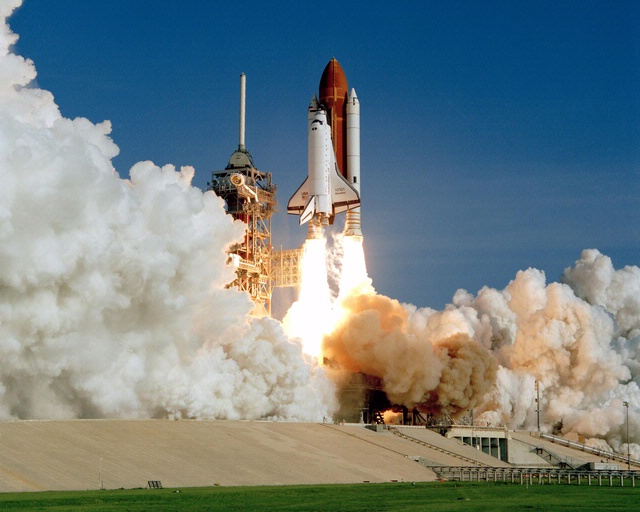
\includegraphics[scale=0.35]{gambar/roketluarangkasa.jpg}

  % Ubah dengan keterangan gambar yang diinginkan
  \caption{Diagram Alir Metode Penelitian}
  \label{fig:metode}
\end{figure}
% what else except nolistsep?

\begin{itemize}[topsep=0pt]
  \item \textbf{Studi Literatur}
  
  Pada tahap ini dilakukan riset studi literatur mengenai konsep 
  dan permasalahan - permasalahan yang sudah ada terkait DISC, 
  Apache Spark, Titian, DistilGPT2, dan FastAPI. Studi literatur didapatkan melalui buku, internet, jurnal penelitian, dan materi-materi kuliah yang berkaitan dengan metode yang akan digunakan.

  \item \textbf{Perancangan Arsitektur Sistem}
  
  \begin{figure}[H]
    \centering
    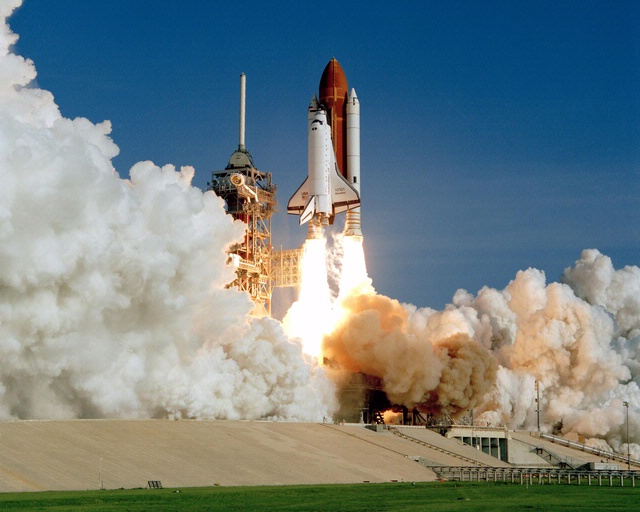
\includegraphics[scale=0.35]{gambar/roketluarangkasa.jpg}
  
    % Ubah dengan keterangan gambar yang diinginkan
    \caption{Rancangan Arsitektur Sistem}
    \label{fig:arsitektur}
  \end{figure}
  
  Tahap perancangan arsitektur sistem pada penelitian ini 
  dilakukan dengan mengombinasikan dasar teori pada bab 2. 
  Perancangan metode akan dimulai dari proses \emph{pre-training}
  terhadap model DistilGPT2 menggunakan baris dataset random dari 
  dataset masing-masing \emph{benchmark program} yang akan 
  diuji. Kemudian program tersebut akan diberikan parameter tertentu 
  agar dapat menghasilkan output yang bermasalah. Setelah itu,
  dengan menggunakan Titian, akan dilakukan proses \emph{provenance data}
  untuk mendapatkan nilai awal dari baris dataset yang menyebabkan
  keluaran yang mencurigakan tersebut. 
  Setelah itu, dilakukan proses re-training lagi terhadap
  model DistilGPT2 menggunakan baris dataset penyebab kesalahan
  tersebut yang kemudian dilakukan proses \emph{generate input}
  baru yang menginduksi kesalahan pada program tersebut dengan jumlah
  yang seminimal mungkin dapat dianalisis oleh \emph{developer}. 
  Hasil dari proses ini kemudian akan dijalankan kembali menggunakan
  program yang sama untuk melihat apakah program tersebut masih
  menghasilkan keluaran yang bermasalah atau tidak.
  Alur keseluruhan proses tersebut dapat dilihat pada 
  Gambar \ref{fig:arsitektur}.

  \item \textbf{Perancangan Metode Generate Input}
  
% endpoint API with FastAPI
% list-model
% - return current, name list

% use-model
% - change current
% —if(not in list)
% 	- make new from base
% - return status

% retrain
% - retrain the model
% - return status

% generate
% - return generate

% reset
% - reset the current from base
% - return status

% delete
% - delete folder current
% - return status

  
  \begin{figure}[H]
    \centering
    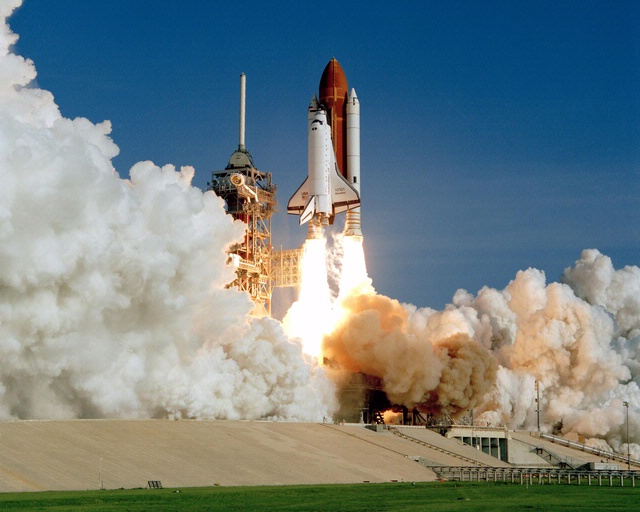
\includegraphics[scale=0.35]{gambar/roketluarangkasa.jpg}
  
    % Ubah dengan keterangan gambar yang diinginkan
    \caption{Rancangan Metode Generate Input}
    \label{fig:generateinput}

  \end{figure}
  
  Tahap perancangan metode generate input dilakukan dengan 
  melakukan proses traning dan re-training terhadap 
  DistilGPT2 model. Proses ini dilakukan dengan membuat sebuah
  API dengan menggunakan FastAPI yang dapat diakses oleh pengguna. 
  API ini akan memiliki beberapa endpoint yang dapat digunakan 
  oleh pengguna untuk melakukan proses \emph{generate input} baru, 
  \emph{re-training new model}, dan \emph{reset model}. Proses 
  penggunaan API ini dilakukan dalam dua tahap, yaitu \emph{local} 
  dan \emph{cloud} milik Amazon Web Service (AWS).
  Tahap ini dapat ditunjukkan melalui Gambar \ref{fig:generateinput}.

  \item \textbf{Pengembangan Sistem}
  
  Pengembangan sistem dilakukan dengan menerapkan algoritma 
  solusi yang dirancang pada subbab perancangan arsitektur 
  sistem dan perancangan metode generate input. Untuk API 
  yang dihasilkan pada perancangan metode generate input 
  akan menggunakan bahasa pemrograman python, sedangkan 
  untuk sistem secara keseluruhan akan menggunakan bahasa 
  pemrograman Scala. Kode program penelitian ini dirancang 
  untuk dapat dipasangkan ke sebuah program yang merupakan 
  program target dilakukannya proses debugging dan generate 
  test input di sistem DISC Apache Spark. Pada saat program 
  target tersebut dijalankan, program pada penelitian ini akan 
  memonitor data input, melakukan re-training model terhadap 
  data yang benar, dan akan melakukan proses generate test 
  input baru untuk menggantikan test input yang bermasalah. 

  \item \textbf{Analisis Kinerja Sistem}
  
  Analisis kinerja sistem yang akan dilakukan pada penelitian ini ada dua, yaitu yaitu pada proses pemisahan dataset dan pada proses generate dataset baru. Analisis kinerja sistem pada proses pemisahan dataset dilakukan dengan menghitung nilai accuracy pada sejumlah program yang akan ditargetkan di mana masing-masing datasetnya akan dilabeli dari awal antara data yang benar dan data yang bermasalah. Untuk analasis kinerja sistem pada proses generate dataset baru dilakukan dengan menghitung persentase dataset benar yang berhasil digenarate oleh model ditiap iterasinya. Proses penentuan apakah dataset baru benar atau bermasalah akan dilakukan secara manual dengan melihat dataset yang telah ada.

  \item \textbf{Penyusunan Laporan Tugas Akhir}
  
  Tahap ini merupakan tahap akhir dari penelitian ini yaitu penyusunan laporan dalam bentuk buku tugas akhir yang menjelaskan dasar teori dan metode yang digunakan dalam tugas akhir ini serta hasil implementasi yang telah dibuat. Sistematika penulisan buku tugas akhir secara garis besar antara lain:

  \begin{enumerate}[topsep=0pt]
    \item Pendahuluan
    \begin{enumerate}[topsep=0pt]
      \item Latar Belakang
      \item Rumusan Masalah
      \item Batasan Masalah
      \item Tujuan
      \item Manfaat
    \end{enumerate}
    \item Tinjauan Pustaka
    \item Metodologi
    \item Hasil dan Pembahasan
    \item Kesimpulan dan Saran
    \item Daftar Pustaka
  \end{enumerate}
\end{itemize}

\section{Peralatan Pendukung}
\label{sec:peralatan pendukung}

Terdapat beberapa peralatan hardware dan software pendukung yang digunakan untuk pengembangan sistem pada Tugas Akhir ini yang dapat dilihat sebagai berikut:
\begin{itemize}[topsep=0pt]
  \item Hardware
  \begin{enumerate}[topsep=0pt]
    \item Laptop MacBook Pro M2
  \end{enumerate}
  \item Software
  \begin{enumerate}[topsep=0pt]
    \item Google Colaboratory
    \item Visual Studio Code
    \item IntelliJ IDEA CE
    \item HuggingFace
    \item Amazon Web Service EC2
  \end{enumerate}
\end{itemize}
\section{Implementasi}
\label{sec:implementasi}
Tujuan utama dari penelitian ini adalah menghasilkan data 
yang menyebabkan kesalahan dalam jumlah yang dapat dengan 
mudah dianalisis oleh developer. 
Gambar \ref{fig:alur kerja teknik} merangkum alur 
kerja teknik kami. Teknik ini dimulai 
dengan penyesuaian awal arsitektur \emph{generative LLM} yang 
sudah dilatih sebelumnya menggunakan sampel acak dari data. 
LLM ini di-host di server langsung dan diakses melalui API 
khusus yang dijelaskan di Tabel \ref{tab:api}. Ketika ditemukan eksekusi 
program yang salah, penelitian kami menggunakan Titain, sebuah 
\emph{provenance engine}, untuk mendapatkan serangkaian baris yang 
mencurigakan. Sampel data yang dilatih ini memiliki 
persentase lebih tinggi dari baris yang menyebabkan kesalahan, 
yang kemudian digunakan untuk lebih menyesuaikan generative 
LLM, sehingga model ini mempelajari pola dasar dari input yang 
menyebabkan kesalahan dan cenderung menghasilkan baris 
yang salah. Akhirnya, dengan menggunakan model ini, 
kami mendorongnya untuk menghasilkan 
sampel baris, secara bertahap meningkatkan jumlah baris 
yang dihasilkan hingga \emph{bug} tersebut terdeteksi kembali.
Dalam membuat Tugas Akhir ini, terdapat beberapa proses 
yang perlu dilakukan sesuai pada gambar \ref{fig:diagram alir implementasi}

\begin{figure}[H]
  \centering
  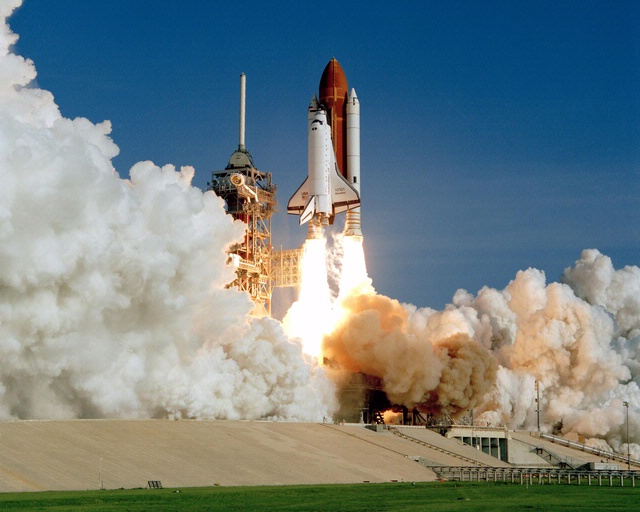
\includegraphics[scale=0.35]{gambar/roketluarangkasa.jpg}

  % Ubah dengan keterangan gambar yang diinginkan
  \caption{Alur Kerja Teknik}
  \label{fig:alur kerja teknik}
\end{figure}

\begin{table}[H]
  \centering
  \caption{Tabel API}
  \begin{tabular}{|c|c|}
    \hline
    \textbf{API} & \textbf{Deskripsi} \\
    \hline
    \texttt{GET /generate} & Menghasilkan input yang menyebabkan kesalahan \\
    \hline
    \texttt{POST /retrain} & Melatih model dengan data yang benar \\
    \hline
  \end{tabular}
  \label{tab:api}
\end{table}

\begin{figure}[H]
  \centering
  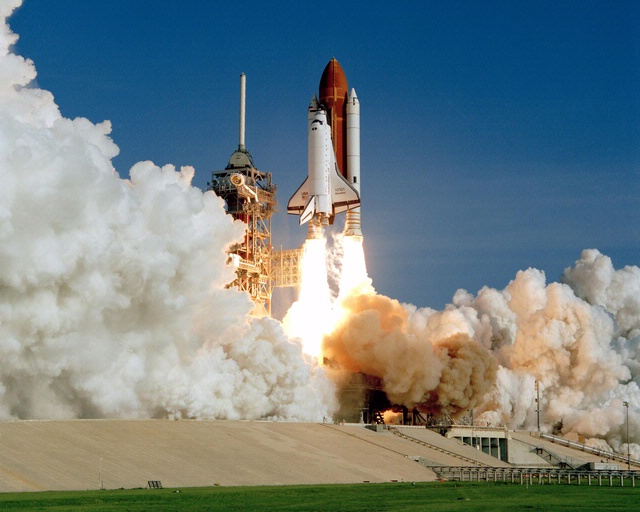
\includegraphics[scale=0.35]{gambar/roketluarangkasa.jpg}

  % Ubah dengan keterangan gambar yang diinginkan
  \caption{Diagram Alir Rencana Implementasi dan Uji Coba}
  \label{fig:diagram alir implementasi}
\end{figure}

\subsection{Mengambil Input yang Menimbulkan Kesalahan dari Eksekusi yang Salah}
\label{sec:mengambil input}

Alat kami pertama-tama menggunakan \emph{provenance tool} 
seperti Titian untuk mendapatkan sampel input yang bias 
terhadap baris-baris yang menginduksi kesalahan dalam eksekusi 
program tertentu. Ketika analis data mengeksekusi program 
dengan data asli, alat kami menggunakan \emph{API call} 
{\tt LLM\_pretrain(orig\_data\_path)} untuk memberikan data 
awal ke server \emph{LLM}. Tujuan dari data ini adalah untuk 
membiasakan \emph{LLM} dengan format dan skema data. 
Perlu dicatat bahwa karena \emph{LLM} menggunakan 
\emph{pre-trained weights} dari GPT-2, tidak diperlukan 
sejumlah besar data untuk dapat menghasilkan baris dengan 
format yang diharapkan. Akibatnya, waktu pelatihan untuk 
langkah ini relatif singkat.

Ketika eksekusi program menghasilkan keluaran yang 
mencurigakan, analis dapat menentukan aturan filter 
menggunakan \emph{Titian's API} untuk mengidentifikasi 
kemungkinan penyebab keluaran yang salah. Data penyebab 
yang dikembalikan oleh Titian bisa sangat besar sehingga 
tidak mungkin dianalisis oleh pengembang manusia, misalnya, 
hingga jutaan baris. Wawasan kami adalah bahwa meskipun data 
penyebabnya besar, inti dari kesalahan dapat ditangkap dalam 
beberapa baris saja. Model bahasa modern adalah alat yang 
berguna untuk menangkap pola-pola yang menginduksi kesalahan 
dari sampel bias yang dikembalikan oleh Titian.

\subsection{Melatih Model Bahasa Pembangkitan Input yang Menginduksi Kesalahan Secara Offline}
\label{sec:melatih model}

Setelah sekumpulan baris potensial yang menyebabkan keluaran 
yang salah diperoleh, alat kami menggunakan \emph{API call} 
{\tt LLM\_pretrain(faulty\_sample)} untuk melatih ulang model 
dengan data yang dicurigai dan membiasakannya untuk 
menghasilkan input yang menginduksi kesalahan. \emph{LLM} 
mengambil baris-baris ini dan menerapkan proses pelatihan 
awal sekali lagi menggunakan baris-baris yang salah yang 
disediakan.

\subsection{Pembuatan Input yang Menginduksi Kesalahan secara Ringkas}
\label{sec:pembuatan input}

Dengan menggunakan model yang bias, alat kami dapat 
menghasilkan input baru yang menginduksi kesalahan untuk 
mereproduksi gejala kesalahan yang sama dengan data yang 
jauh lebih sedikit. Karena model yang dilatih adalah 
\emph{generative LLM}, kami dapat menggunakan 
\emph{API call} {\tt LLM\_generate(N)} untuk menghasilkan 
N baris data. Idealnya, N yang dibutuhkan untuk mereproduksi 
kesalahan harus cukup kecil agar mudah dianalisis oleh 
programmer manusia. Secara analitis, menentukan nilai N 
sangat sulit, jika tidak bisa dibilang mustahil. Oleh 
karena itu, alat kami mengambil pendekatan iteratif. 
Alat ini memulai dengan memanggil {\tt LLM\_generate(1)} 
dan mengeksekusi program menggunakan baris yang dihasilkan. 
Jika gejala kesalahan terproduksi, loop berhenti. Jika tidak, 
alat ini meningkatkan N secara logaritmik hingga kesalahan 
terproduksi. Jika alat ini tidak dapat mereproduksi kesalahan 
dalam jumlah iterasi yang ditentukan oleh pengguna, loop akan 
dihentikan dan alat melaporkan kegagalan untuk mereproduksi 
kesalahan.

\subsection{Mengunggah API ke Layanan Cloud}
\label{sec:mengunggah api}

Setelah model telah berhasil dilatih untuk menghasilkan 
input yang menginduksi kesalahan dan diuji untuk memastikan 
efektivitasnya, langkah selanjutnya adalah mengunggah 
\emph{API} ke layanan \emph{cloud}. Mengunggah \emph{API} 
ke layanan \emph{cloud} memungkinkan akses yang mudah dan 
skalabilitas untuk pengguna di berbagai lokasi. Dengan 
menggunakan \emph{API} yang diunggah ke \emph{cloud}, 
pengembang dapat mengotomatisasi proses deteksi dan 
reproduksi kesalahan tanpa perlu mengelola infrastruktur 
secara langsung. Layanan \emph{cloud} juga menyediakan 
sumber daya yang diperlukan untuk menangani permintaan 
\emph{API} dalam jumlah besar, memastikan bahwa alat 
tetap responsif dan efisien bahkan di bawah beban kerja 
yang tinggi. Langkah ini melibatkan konfigurasi server 
\emph{cloud} untuk menjalankan \emph{LLM} dan mengatur 
\emph{endpoint API} untuk menerima dan memproses permintaan 
dari pengguna, memungkinkan integrasi yang mulus dengan 
berbagai sistem dan aplikasi.

% Contoh pembuatan potongan kode
\begin{lstlisting}[
  language=C++,
  caption={Program halo dunia.},
  label={lst:halodunia}
]
#include <iostream>

int main() {
    std::cout << "Halo Dunia!";
    return 0;
}
\end{lstlisting}

\lipsum[2-3]

% Contoh input potongan kode dari file
\lstinputlisting[
  language=Python,
  caption={Program perhitungan bilangan prima.},
  label={lst:bilanganprima}
]{program/bilangan-prima.py}


\lstinputlisting[
  caption={Program perhitungan bilangan prima.},
  label={lst:contoh-pseudocode}
]{program/contoh-pseudocode.txt}

\cleardoublepage

% Bab 4 hasil dan pembahasan
\chapter{HASIL DAN PEMBAHASAN}
\label{chap:hasildanpembahasan}

Pada penelitian ini dipaparkan \lipsum[1][1-5]

\section{Hasil Eksperimen}
\label{sec:hasilpengujian}

\subsection{Lingkungan Pengujian}
\label{subsec:lingkunganpengujian}

Untuk menjawab rumusan masalah yang diajukan oleh penelitian ini,
kami melakukan eksperimen pada aplikasi \emph{benchmark}
DISC yang telah ada, yang diadaptasi dari penelitian sebelumnya
tentang \emph{debugging} dan pengujian aplikasi DISC. \emph{Benchmark}
ini merupakan campuran dari alur kerja \emph{big data} yang
terinspirasi dari SQL dan dunia nyata. Aplikasi-aplikasi
ini juga dilengkapi dengan kesalahan yang sudah disuntikkan
sebelumnya yang mewakili \emph{bug} dunia nyata. Secara total,
kami menjalankan eksperimen pada 16 aplikasi \emph{benchmark}
DISC yang bermasalah. Aplikasi-aplikasi ini dilengkapi
dengan skrip pembuatan data yang memungkinkan data
dihasilkan dengan faktor skala, mirip dengan
\emph{benchmark} TPC-DS. Kami menggunakan laptop standar
untuk menerapkan Apache Spark 2.0.0 karena Titian
awalnya dirancang untuk Apache Spark 2.0.0. Namun,
FISUM sepenuhnya kompatibel dengan versi terbaru dari
Spark karena tidak memerlukan instrumen apa pun dalam
kode sumber Apache Spark. 

Berikut adalah deskripsi dari ke 16 aplikasi \emph{benchmark}
yang digunakan dalam penelitian ini:
\begin{enumerate}
      \item \emph{\textbf{Age Analysis}} \\
            Program \emph{age analysis} digunakan untuk mengklasifikasikan penduduk di sebuah area dengan kode pos "90024" sesuai dengan umur mereka. 
            Dalam program ini, Titian diaplikasikan untuk mendeteksi input yang memiliki data penduduk yang memiliki umur lebih dari 50.
            Adapun contoh dataset yang digunakan dapat 
            dilihat pada Tabel \ref{tb:ageanalysisdataset}.

            \begin{longtable}{|c|c|c|}
                  \caption{Contoh Dataset Age Analysis.}
                  \label{tb:ageanalysisdataset} \\
                  \hline
                  \rowcolor[HTML]{C0C0C0}
                  \textbf{Kode Pos} & \textbf{Umur} & \textbf{Jumlah} \\
                  \hline
                  90024 & 20 & 1000 \\
                  90024 & 30 & 2000 \\
                  90024 & 159 & 3000 \\
                  \hline
            \end{longtable}
      
      \item \emph{\textbf{Commute Type}} \\
            Program \emph{commute type} menggunakan dataset berupa kode pos area A, kode pos area B, jarak, serta waktu yang ditempuh. Selanjutnya, program akan mengolah jarak dan waktu menjadi kecepatan yang terjadi dalam menempuh perjalanan dari area A ke B. Dari data kecepatan tersebut, program akan mengklasifikasikan ke dalam tiga kategori, yaitu sebagai berikut:
            \begin{itemize}
                  \item kecepatan $ > $ 40 = \emph{car}
                  \item kecepatan $ > $ 15 = \emph{public}
                  \item kecepatan $ \leq $ 15 = \emph{on foot}
            \end{itemize}
            Namun, dari ketiga kategori tersebut, untuk kecepatan $ > $ 100 dikategorikan sebagai kesalahan input karena mobil tidak akan melebihi batas kecepatan tersebut.
            Adapun contoh dataset yang digunakan dapat 
            dilihat pada Tabel \ref{tb:commutetypedataset}.

            \begin{longtable}{|c|c|c|c|c|}
                  \caption{Contoh Dataset Commute Type.}
                  \label{tb:commutetypedataset} \\
                  \hline
                  \rowcolor[HTML]{C0C0C0}
                  \textbf{\#} & \textbf{Kode Pos A} & \textbf{Kode Pos B} & \textbf{Jarak} & \textbf{Waktu} \\
                  sr & 90002 & 90017 & 1501 & 100 \\
                  sr & 90098 & 90077 & 2106 & 37 \\
                  sr & 90079 & 90009 & 7009 & 116 \\
                  \hline
            \end{longtable}

      \item \emph{\textbf{Commute Type Full}} \\
      % sr,90002,90017,1501,100
      % sr,90098,90077,2106,37
      % sr,90079,90009,7009,116
            Program \emph{commute type full} menggunakan 2 dataset, yaitu \emph{trips} dan \emph{locations}. Dataset \emph{trips} berupa kode pos area A, kode pos area B, jarak, serta waktu yang ditempuh. Sedangkan, dataset kedua yang digunakan adalah \emph{locations}, dataset ini berisi lokasi dari sebuah kode pos. Selanjutnya, program akan menggabungkan kedua dataset apabila ada kesamaan pada kode pos. Kemudian, program akan mengolah jarak dan waktu menjadi kecepatan yang terjadi dalam menempuh perjalanan dari kota A ke B. Dari data kecepatan tersebut, program akan mengklasifikasikan ke dalam tiga kategori, yaitu sebagai berikut:
            \begin{itemize}
                  \item kecepatan $ > $ 40 = \emph{car}
                  \item kecepatan $ > $ 15 = \emph{public}
                  \item kecepatan $ \leq $ 15 = \emph{on foot}
            \end{itemize}
            Pada program ini, Titian bekerja untuk mendeteksi input yang dianggap salah, yaitu yang memiliki ID lokasi kurang dari sama dengan 1000.
            Adapun contoh dataset yang digunakan dapat 
            dilihat pada Tabel \ref{tb:commutetypefulldataset}.

            \begin{longtable}{|c|c|c|c|c|}
                  \caption{Contoh Dataset Commute Type Full.}
                  \label{tb:commutetypefulldataset} \\
                  \hline
                  \rowcolor[HTML]{C0C0C0}
                  \textbf{\#} & \textbf{Kode Pos A} & \textbf{Kode Pos B} & \textbf{Jarak} & \textbf{Waktu} \\
                  sr & 90002 & 90017 & 1501 & 100 \\
                  sr & 90098 & 90077 & 2106 & 37 \\
                  sr & 90079 & 90009 & 7009 & 116 \\
                  \hline
            \end{longtable}
      
      \item \emph{\textbf{Customers}} \\
      % s"""$oid,$cid,$time,$item"""
      % order651,888,78895039,item797864327
      % order515,481,1701910512,item765935155
      % order531,24,1171869537,item354502894
            Program \emph{customers} akan mengolah dua dataset, yaitu dataset \emph{customers\_data} dan \emph{orders\_data}. Kedua dataset ini akan digabungkan apabila memiliki kesamaan data dan akan menganalisis customer mana yang setidaknya sudah membuat 3 kali pembelian dalam jangka waktu yang sudah ditentukan. Dalam program ini, Titian hanya mencari input data yang memiliki order ID kurang dari 100 dan dinyatakan sebagai input yang salah.
            Adapun contoh dataset yang digunakan dapat 
            dilihat pada Tabel \ref{tb:customersdataset}.

            \begin{longtable}{|c|c|c|c|}
                  \caption{Contoh Dataset Customers.}
                  \label{tb:customersdataset} \\
                  \hline
                  \rowcolor[HTML]{C0C0C0}
                  \textbf{ID Order} & \textbf{ID Pelanggan} & \textbf{Waktu} & \textbf{Item} \\
                  \hline
                  order651 & 888 & 78895039 & item797864327 \\
                  order515 & 481 & 1701910512 & item765935155 \\
                  order531 & 24 & 1171869537 & item354502894 \\
                  \hline
            \end{longtable}
            
      \item \emph{\textbf{Delays}} \\
      % s"""$tripId,$a,$d,$r"""
      % trip63811,2128804415,1221732780,route56
      % trip46102,1777873050,482274628,route49
      % trip38403,140174683,1960456261,route64
            \emph{Delays} adalah program yang digunakan untuk mencari data bus yang mengalami keterlambatan (\emph{delay}). Dataset yang digunakan ada 2, yaitu \emph{dataStation1} dan \emph{dataStation2}. Kedua dataset ini memiliki waktu keberangkatan dan tiba dari setiap ID perjalanan. Kemudian, kedua dataset digabungkan apabila memiliki kesamaan data. Selanjutnya, program akan menghitung keterlambatan dari waktu keberangkatan dan tiba dari setiap elemen. Dalam program ini, Titian diterapkan untuk mencari input data yang memiliki waktu keberangkatan lebih besar daripada waktu tiba, karena dinyatakan sebagai ketidakmungkinan dalam kasus nyata.
            Adapun contoh dataset yang digunakan dapat 
            dilihat pada Tabel \ref{tb:delaysdataset}.

            \begin{longtable}{|c|c|c|c|}
                  \caption{Contoh Dataset Delays.}
                  \label{tb:delaysdataset} \\
                  \hline
                  \rowcolor[HTML]{C0C0C0}
                  \textbf{ID Perjalanan} & \textbf{Waktu Berangkat} & \textbf{Waktu Tiba} & \textbf{Rute} \\
                  \hline
                  trip63811 & 2128804415 & 1221732780 & route56 \\
                  trip46102 & 1777873050 & 482274628 & route49 \\
                  trip38403 & 140174683 & 1960456261 & route64 \\
                  \hline
            \end{longtable}

      \item \emph{\textbf{Delivery Faults}} \\
      % s"""$did,$cid,$vend,$rating"""
      % dlvry96998,cust43114,vend65077,5
      % dlvry16209,cust64119,vend8516,5
      % dlvry89647,cust10882,vend3328,5
            \emph{Delivery Faults} adalah program yang dapat mencari pengiriman mana yang buruk dari rating yang dimilikinya. Titian diterapkan dalam program ini untuk mendeteksi input yang memiliki rating lebih dari 5.
            Adapun contoh dataset yang digunakan dapat 
            dilihat pada Tabel \ref{tb:deliveryfaultsdataset}.

            \begin{longtable}{|c|c|c|c|}
                  \caption{Contoh Dataset Delivery Faults.}
                  \label{tb:deliveryfaultsdataset} \\
                  \hline
                  \rowcolor[HTML]{C0C0C0}
                  \textbf{ID Pengiriman} & \textbf{ID Pelanggan} & \textbf{ID Vendor} & \textbf{Rating} \\
                  \hline
                  dlvry96998 & cust43114 & vend65077 & 5 \\
                  dlvry16209 & cust64119 & vend8516 & 5 \\
                  dlvry89647 & cust10882 & vend3328 & 5 \\
                  \hline
            \end{longtable}

      \item \emph{\textbf{External Call}} \\
      % Teks
      % This is a sentence
      % This not a sentence
      % This is a word
      % My name is black
      % I am a student
            Program \emph{external call} memiliki tujuan untuk mencari kata yang sering muncul dalam suatu dataset, cara kerjanya adalah menjumlahkan setiap kata yang sama, kemudian apabila kata tersebut muncul lebih dari 1 maka dinyatakan sebagai kata yang sering muncul. Dalam program ini, Titian hanya akan melacak data yang jarang muncul yaitu yang memiliki jumlah kemunculan kurang dari atau sama dengan 1.
            Adapun contoh dataset yang digunakan dapat 
            dilihat pada Tabel \ref{tb:externalcalldataset}.

            \begin{longtable}{|c|}
                  \caption{Contoh Dataset External Call.}
                  \label{tb:externalcalldataset} \\
                  \hline
                  \rowcolor[HTML]{C0C0C0}
                  \textbf{Teks} \\
                  \hline
                  This is a sentence \\
                  This not a sentence \\
                  This is a word \\
                  My name is black \\
                  I am a student \\
                  \hline
            \end{longtable}

      \item \emph{\textbf{Find Salary}} \\
      % $522224
      % $415728
      % $501565
      % $820638
            \emph{Find salary} menggunakan satu data set yang berisi nominal gaji setiap orang, Program ini akan mencari gaji yang kurang dari 300. Kemudian, Titian diterapkan hanya untuk mendeteksi gaji yang lebih besar atau sama dengan 300.
            Adapun contoh dataset yang digunakan dapat 
            dilihat pada Tabel \ref{tb:findsalarydataset}.

            \begin{longtable}{|c|}
                  \caption{Contoh Dataset Find Salary.}
                  \label{tb:findsalarydataset} \\
                  \hline
                  \rowcolor[HTML]{C0C0C0}
                  \textbf{Gaji} \\
                  \hline
                  \$522224 \\
                  \$415728 \\
                  \$501565 \\
                  \$820638 \\
                  \hline
            \end{longtable}

      \item \emph{\textbf{Flight Distance}} \\
      % s"""$airportCode,$airportName,$airportName2,$long,$lat,$continent"""
      % LAX,2n8Hga8ICV,MpQ4TQZrHs,151.3466,-68.5339,PRkqAcg4rZ
      % LAS,hOvx8HlmGI,ke7IhMxWmx,123.0983,5.819,zQ6Zrv9bgQ
      % LAS,AJSAZYp44p,lJW9lm2npx,135.2637,-25.0603,Fter9EB1Vd
      % LAS,3L4mwHv6Wr,pkUt6axm1Y,176.4615,23.2344,wcb4CeYYo7
      % LAS,eRUZDr9FqE,XXuxIq7gGT,-134.0949,10.8214,SxtFuOA1xS
            Program \emph{flight distance} adalah program yang dapat mengolah data dari dua dataset, yaitu \emph{flights\_data} dan \emph{airports\_data}, yang mana hasil akhirnya adalah akan mengetahui jarak dari keberangkatan dan tiba dari setiap penerbangan. 
            Terdapat banyak input yang berupa lokasi bandara, kami gunakan input yang memiliki lokasi berkode "LAS" dan "LAX" sebagai input yang salah. Kemudian, input tersebut akan dilacak dengan Titian.
            Adapun contoh dataset yang digunakan dapat 
            dilihat pada Tabel \ref{tb:flightdistancedataset}.

            \begin{longtable}{|p{0.12\linewidth}|p{0.17\linewidth}|p{0.17\linewidth}|c|c|c|}
                  \caption{Contoh Dataset Flight Distance.}
                  \label{tb:flightdistancedataset} \\
                  \hline
                  \rowcolor[HTML]{C0C0C0}
                  \raggedright{\textbf{Kode Bandara}} & \raggedright{\textbf{Nama Bandara Asal}} & \raggedright{\textbf{Nama Bandara Tujuan}} & \textbf{Long} & \textbf{Lat} & \textbf{Benua} \\
                  \hline
                  LAX & 2n8Hga8ICV & MpQ4TQZrHs & 151.3466 & -68.5339 & PRkqAcg4rZ \\
                  LAS & hOvx8HlmGI & ke7IhMxWmx & 123.0983 & 5.819 & zQ6Zrv9bgQ \\
                  LAS & AJSAZYp44p & lJW9lm2npx & 135.2637 & -25.0603 & Fter9EB1Vd \\
                  LAS & 3L4mwHv6W & pkUt6axm1Y & 176.4615 & 23.2344 & wcb4CeYYo7 \\
                  LAS & eRUZDr9FqE & XXuxIq7gGT & -134.0949 & 10.8214 & SxtFuOA1xS \\
                  \hline
            \end{longtable}
            
      \item \emph{\textbf{Income Aggregation}} \\
      % \item  s"""$zip,$age,$r"""
      % 90084,11,9248
      % 90080,12,6140
      % 90014,15,1199
      % 90031,53,7558
      % 90017,17,7820
            \emph{Income aggregation} menggunakan dataset yang terdiri dari kode pos, umur, dan jumlah income. Program ini digunakan untuk mengklasifikasikan income masing-masing orang dari umurnya. Lalu, Titian akan digunakan untuk melacak asal usul data yang memiliki kode pos 90024.
            Adapun contoh dataset yang digunakan dapat 
            dilihat pada Tabel \ref{tb:incomeaggregationdataset}.

            \begin{longtable}{|c|c|c|}
                  \caption{Contoh Dataset Income Aggregation.}
                  \label{tb:incomeaggregationdataset} \\
                  \hline
                  \rowcolor[HTML]{C0C0C0}
                  \textbf{Kode Pos} & \textbf{Umur} & \textbf{Pendapatan} \\
                  \hline
                  90024 & 11 & 9248 \\
                  90080 & 12 & 6140 \\
                  90014 & 15 & 1199 \\
                  90031 & 53 & 7558 \\
                  90017 & 17 & 7820 \\
                  \hline
            \end{longtable}

      \item \emph{\textbf{Inside Circle}} \\
      % s"""$x,$y,$r"""
      % 49,26,711
      % 7,26,1870
      % 79,62,845
      % 64,65,1768
      % 2,45,611
            \emph{Inside circle} digunakan untuk menghitung data 3 bilangan random untuk memastikan apakah bilangan x dan y ada dalam radius z. Kegagalan atau kesalahan input yang akan dicari dalam program ini adalah data yang memiliki ukuran x dan y yang berada di luar radius z, yang mana tidak ada di dalam lingkaran.
            Adapun contoh dataset yang digunakan dapat 
            dilihat pada Tabel \ref{tb:insidecircledataset}.

            \begin{longtable}{|c|c|c|}
                  \caption{Contoh Dataset Inside Circle.}
                  \label{tb:insidecircledataset} \\
                  \hline
                  \rowcolor[HTML]{C0C0C0}
                  \textbf{X} & \textbf{Y} & \textbf{Radius} \\
                  \hline
                  49 & 26 & 711 \\
                  7 & 26 & 1870 \\
                  79 & 62 & 845 \\
                  64 & 65 & 1768 \\
                  2 & 45 & 611 \\
                  \hline
            \end{longtable}

      \item \emph{\textbf{Loan Type}} \\
      % s"""$id,$years,$rate,$name"""
      % 9947,40,0.68,2VOJMwmAvI
      % 1528,26,0.1958,HX3TUb4BHP
      % 4543,26,0.4936,kFap4MRPKF
      % 2960,49,0.4724,sobTpzhCj1
      % 9709,45,0.2774,vgSAOZGUOe
            \emph{Loan type} adalah program yang menentukan tipe pinjaman untuk setiap orang yang ada dalam dataset. Dataset terdiri dari id, years, rate, dan name. Tipe pinjaman tersebut ditentukan oleh id pinjaman dan tahun yang dibutuhkan. Dalam hal ini, Titian hanya akan melacak data yang memiliki tahun lebih dari 30 sebagai data yang tidak valid.
            Adapun contoh dataset yang digunakan dapat 
            dilihat pada Tabel \ref{tb:loantypedataset}.

            \begin{longtable}{|c|c|c|c|}
                  \caption{Contoh Dataset Loan Type.}
                  \label{tb:loantypedataset} \\
                  \hline
                  \rowcolor[HTML]{C0C0C0}
                  \textbf{ID} & \textbf{Tahun} & \textbf{Rate} & \textbf{Nama} \\
                  \hline
                  9947 & 40 & 0.68 & 2VOJMwmAvI \\
                  1528 & 26 & 0.1958 & HX3TUb4BHP \\
                  4543 & 26 & 0.4936 & kFap4MRPKF \\
                  2960 & 49 & 0.4724 & sobTpzhCj1 \\
                  9709 & 45 & 0.2774 & vgSAOZGUOe \\
                  \hline
            \end{longtable}

      \item \emph{\textbf{Movie Rating}} \\
      % s"""$movie,$rating"""
      % dRQe4ozltL,29
      % zsDzE9OsBs,47
      % FWvC1vPmjI,14
      % SUKqG8bhNK,8
      % sVXO7BbstA,7
            Program \emph{movie rating} adalah untuk mencari film yang memiliki rating lebih dari 4, maka dari itu Titian diterapkan untuk mencari data yang memiliki rating dibawah 4 sebagai data yang tidak valid.
            Adapun contoh dataset yang digunakan dapat 
            dilihat pada Tabel \ref{tb:movieratingdataset}.

            \begin{longtable}{|c|c|}
                  \caption{Contoh Dataset Movie Rating.}
                  \label{tb:movieratingdataset} \\
                  \hline
                  \rowcolor[HTML]{C0C0C0}
                  \textbf{Film} & \textbf{Rating} \\
                  \hline
                  dRQe4ozltL & 29 \\
                  zsDzE9OsBs & 47 \\
                  FWvC1vPmjI & 14 \\
                  SUKqG8bhNK & 8 \\
                  sVXO7BbstA & 7 \\
                  \hline
            \end{longtable}

      \item \emph{\textbf{Number Series}} \\
      % s"""$n1,$n2"""
      % 319,429
      % 254,347
      % 481,347
      % 424,253
      % 256,17

            Program ini menghitung jarak antara 2 bilangan berdasarkan \emph{Collatz Conjecture}. Kemudian, Titian akan melacak bilangan yang memiliki jarak tidak sama dengan 25 sebagai data yang tidak valid.
            Adapun contoh dataset yang digunakan dapat 
            dilihat pada Tabel \ref{tb:numberseriesdataset}.

            \begin{longtable}{|c|c|}
                  \caption{Contoh Dataset Number Series.}
                  \label{tb:numberseriesdataset} \\
                  \hline
                  \rowcolor[HTML]{C0C0C0}
                  \textbf{Bilangan 1} & \textbf{Bilangan 2} \\
                  \hline
                  319 & 429 \\
                  254 & 347 \\
                  481 & 347 \\
                  424 & 253 \\
                  256 & 17 \\
                  \hline
            \end{longtable}

      \item \emph{\textbf{Student Grade}} \\
      % s"""$course,$score"""
      % CS428,344
      % CS478,510
      % CS395,349
      % CS430,592
      % CS209,437
            \emph{Student grade} adalah program analisis nilai dari setiap siswa yang mana apabila siswa mendapatkan nilai lebih dari 40 maka statusnya adalah pass, sedangkan siswa yang mendapat nilai kurang dari atau sama dengan 40 maka statusnya adalah fail. Dalam program ini Titian digunakan untuk mencari input data yang memiliki nilai lebih dari 100 karena nilai lebih dari 100 adalah sesuatu yang tidak valid.
            Adapun contoh dataset yang digunakan dapat 
            dilihat pada Tabel \ref{tb:studentgradedataset}.

            \begin{longtable}{|c|c|}
                  \caption{Contoh Dataset Student Grade.}
                  \label{tb:studentgradedataset} \\
                  \hline
                  \rowcolor[HTML]{C0C0C0}
                  \textbf{Mata Pelajaran} & \textbf{Nilai} \\
                  \hline
                  CS428 & 344 \\
                  CS478 & 510 \\
                  CS395 & 349 \\
                  CS430 & 592 \\
                  CS209 & 437 \\
                  \hline
            \end{longtable}

      \item \emph{\textbf{Word Count}} \\
      % This is a sentence
      % This not a sentence
      % This is a word
            \emph{Word count} adalah program untuk menghitung jumlah huruf yang sama dalam suatu dataset. Dalam program ini, Titian digunakan untuk mencari asal-usul data yang memiliki kata "sentence" sebagai input yang tidak valid.
            Adapun contoh dataset yang digunakan dapat 
            dilihat pada Tabel \ref{tb:wordcountdataset}.

            \begin{longtable}{|c|}
                  \caption{Contoh Dataset Word Count.}
                  \label{tb:wordcountdataset} \\
                  \hline
                  \rowcolor[HTML]{C0C0C0}
                  \textbf{Teks} \\
                  \hline
                  This is a sentence \\
                  This not a sentence \\
                  This is a word \\
                  \hline
            \end{longtable}

\end{enumerate}


\subsection{Skenario Uji Coba}
\label{subsec:skenarioujicoba}

Sebelum melakukan pengujian, kami menentukan beberapa 
\emph{variable} yang akan digunakan dalam pengujian ini.
Selain dari ke 16 aplikasi \emph{benchmark} yang digunakan,
kami juga menentukan besar persentase data yang akan
dihasilkan oleh FISUM, yaitu 1\%, 2\%, 5\%, 10\%, 25\%, dan
50\% dari dataset asli. Adapun pengujian yang dilakukan
adalah sebagai berikut:

% item
\begin{itemize}
  \item \emph{\textbf{Fault Detection Capability}} \\
  Untuk menilai apakah \emph{input} yang bermasalah yang 
  dihasilkan oleh FISUM masih mempertahankan kemampuan 
  deteksi kesalahan, kami memisahkan dataset asli 
  menjadi data yang benar dan bermasalah, kemudian 
  menggunakan FISUM untuk merangkum data bermasalah 
  menjadi hanya beberapa baris data saja
  dan membandingkan akurasi deteksi kesalahan antara 
  input asli dan yang diringkas.
  \item \emph{\textbf{Data Reduction}} \\
  Untuk mengukur persentase pengurangan input bermasalah 
  yang dihasilkan oleh FISUM dari dataset yang diberikan, 
  kami menghitung jumlah data bermasalah sebelum dan 
  sesudah peringkasan oleh FISUM dan menentukan persentase 
  pengurangannya di mana dataset baru yang dihasilkan
  tetap memiliki kesalahan yang sama dengan dataset asli.
  \item \emph{\textbf{Data Generation Time}} \\
  Untuk menentukan waktu yang dibutuhkan untuk 
  menghasilkan input bermasalah oleh FISUM, kami 
  mencatat waktu mulai dan selesai proses \emph{generating} data 
  lalu melakukan beberapa kali pengukuran sesuai
  dengan persentase data yang dihasilkan oleh FISUM.
  \item \emph{\textbf{Model Training Time}} \\
  Untuk mengukur waktu yang dibutuhkan untuk melatih 
  tiap model dengan FISUM, kami mencatat waktu mulai 
  dan selesai dari proses pelatihan model menggunakan 
  input yang telah diringkas oleh FISUM, kemudian 
  melakukan beberapa iterasi pada berbagai ukuran 
  dataset untuk menganalisis efektivitas dan efisiensi 
  waktu pelatihan.
\end{itemize}

\section{Pembahasan}
\label{sec:pembahasan}

Dari pengujian yang dilakukan berdasarkan skenario uji coba,
kami mendapatkan hasil yang menarik yang akan kami tampilkan
pada Tabel \ref{tb:HasilPengujian}.
\emph{\textbf{Failing Input}} mewakili jumlah baris 
yang diperoleh setelah menerapkan Titian 
(\emph{data provenance}) pada keluaran yang gagal. 
\emph{\textbf{Data Reduction}} mewakili total jumlah 
baris (ringkasan) yang kami hasilkan dengan FISUM. 
\emph{\textbf{Fault Detection Rate}} mewakili proporsi 
input yang bermasalah di antara total input yang 
dihasilkan oleh FISUM.

\begin{longtable}{|c|p{0.14\linewidth}|p{0.1\linewidth}|p{0.09\linewidth}|r|r|r|r|r|r|c|}
      \caption{Evaluasi Program.}
      \label{tb:HasilPengujian} \\
      \hline
      &  & &  & \multicolumn{6}{|c|}{\textbf{\% Data Reduction (Rows)}} & {\textbf{Fault}} \\
      \textbf{\#} & \textbf{Program} & {\textbf{Program}} & {\textbf{Failing}} & & & & & & & {\textbf{Detection}} \\
      & \textbf{Name} &  {\bf Input} &  {\bf Output} & \textbf{1\%} & \textbf{2\%} & \textbf{5\%} & \textbf{10\%} & \textbf{25\%} & \textbf{50\%}  & {\textbf{Rate}} \\
      & & & & & & & & & & {\textbf{(Average)}} \\
      \hline
      1 & \raggedright{Age Analysis} & 10000 & 94 & 1 & 2 & 5 & 10 & 25 & 50 & 100\% \\
      \hline
      2 & \raggedright{Commute Type} & 10000 & 60 & 1 & 2 & 3 & 6 & 15 & 30 & 100\% \\
      \hline
      3 & \raggedright{Commute Type Full} & 10000 & 138 & 2 & 3 & 7 & 14 & 35 & 69 & 100\% \\
      \hline
      4 & Customers & 10000 & 1044 & 11 & 21 & 53 & 105 & 261 & 522 & 100\% \\
      \hline
      5 & Delays & 10000 & 2508 & 26 & 51 & 126 & 251 & 627 & 1254 & 93\% \\
      \hline
      6 & \raggedright{Delivery Faults} & 10000 & 1559 & 16 & 32 & 78 & 156 & 390 & 780 & 100\% \\
      \hline
      7 & \raggedright{External Call} & 10000 & 10000 & 100 & 200 & 500 & 1000 & 2500 & 5000 & 100\% \\
      \hline
      8 & \raggedright{Find Salary} & 10000 & 9997 & 100 & 200 & 500 & 1000 & 2500 & 4999 & 100\% \\
      \hline
      9 & \raggedright{Flight Distance} & 10000 & 225 & 3 & 5 & 12 & 23 & 57 & 113 & 100\% \\
      \hline
      10 & \raggedright{Income Aggregation} & 10000 & 98 & 1 & 2 & 5 & 10 & 25 & 49 & 100\% \\
      \hline
      11 & Inside Circle & 10000 & 126 & 2 & 3 & 7 & 13 & 32 & 63 & 97.4\% \\
      \hline
      12 & Loan Type & 10000 & 4746 & 48 & 95 & 238 & 475 & 1187 & 2373 & 100\% \\
      \hline
      13 & \raggedright{Movie Rating} & 10000 & 440 & 5 & 9 & 22 & 44 & 110 & 220 & 100\% \\
      \hline
      14 & \raggedright{Number Series} & 10000 & 9734 & 98 & 195 & 487 & 974 & 2434 & 4867 & 100\% \\
      \hline
      15 & \raggedright{Student Grade} & 10000 & 8949 & 90 & 179 & 448 & 895 & 2238 & 4475 & 100\% \\
      \hline
      16 & \raggedright{Word Count} & 10000 & 10000 & 100 & 200 & 500 & 1000 & 2500 & 5000 & 100\% \\
      \hline         
\end{longtable}


% Contoh pembuatan tabel
% \begin{longtable}{|c|c|c|}
%   \caption{Hasil Pengukuran Energi dan Kecepatan}
%   \label{tb:EnergiKecepatan}                                   \\
%   \hline
%   \rowcolor[HTML]{C0C0C0}
%   \textbf{Energi} & \textbf{Jarak Tempuh} & \textbf{Kecepatan} \\
%   \hline
%   10 J            & 1000 M                & 200 M/s            \\
%   20 J            & 2000 M                & 400 M/s            \\
%   30 J            & 4000 M                & 800 M/s            \\
%   40 J            & 8000 M                & 1600 M/s           \\
%   \hline
% \end{longtable}

\subsection{Analisis}
\label{subsec:analisis}

Untuk memberikan gambaran umum dari hasil penelitian kami 
dan menunjukkan manfaat dari penelitian kami, kami membahas 
program \emph{Delays} dari \emph{benchmark} aplikasi kami. 
Program Delays menganalisis data waktu kedatangan dan 
keberangkatan bus untuk mengetahui rute bus mana yang 
mengalami keterlambatan. Contoh data untuk program ini 
ditunjukkan pada Subbab \ref{subsec:lingkunganpengujian}.
Kolom \emph{RouteID} adalah pengenal unik untuk rute 
bus tertentu, kolom \emph{Departure Timestamp} adalah 
\emph{UNIX timestamp} dalam detik yang mewakili waktu 
keberangkatan bus dari stasiun bus awal pada rute tersebut. 
Kolom \emph{Arrival Timestamp} adalah \emph{UNIX timestamp} 
dalam detik yang mewakili waktu kedatangan bus kembali 
ke stasiun bus setelah menyelesaikan rutenya.

Program yang ditulis oleh pengguna mengasumsikan bahwa 
waktu keberangkatan bus akan selalu lebih kecil dari 
waktu kedatangan. Secara logis, asumsi ini benar, 
tetapi karena kesalahan entri data sesekali, asumsi 
ini dapat dilanggar yang menyebabkan hasil analisis 
yang salah.

\textbf{Hasil dengan Titian}: Ketika analis data yang 
menulis program tersebut mengamati bahwa program mereka 
menghasilkan keluaran yang mencurigakan, mereka 
menggunakan Titian, sebuah \emph{data provenance} 
yang dapat bekerja mundur dari keluaran untuk menemukan 
input mana yang bertanggung jawab atas keluaran 
mencurigakan, untuk menemukan baris penyebab. 
Titian mengembalikan 2508 baris yang bisa bertanggung 
jawab atas keluaran tersebut. Namun, jumlah baris ini 
terlalu banyak untuk dianalisis secara manual oleh 
analis data, yang menyebabkan waktu debugging lebih lama.

\textbf{Menggunakan FISUM}: Sekarang analis data 
menggunakan FISUM untuk mengetahui apa yang menyebabkan 
keluaran mencurigakan. FISUM menggunakan Titian bersama 
dengan \emph{LLM backend} untuk meringkas 
\emph{fault-inducing input}. Akhirnya, FISUM mengembalikan 
26 baris yang merupakan calon penyebab 
\emph{fault-inducing input}, $\approx 1\%$ dari ukuran 
keluaran Titian.

\subsection{Evaluasi}
\label{subsec:evaluasi}

Untuk mengevaluasi efektivitas FISUM, kami melakukan uji
coba pada 16 aplikasi \emph{benchmark} yang bermasalah
sesuai dengan skenario uji coba yang telah ditentukan
sebelumnya. Berikut adalah hasil pengujian yang kami:

% item
\begin{itemize}
  \item \emph{\textbf{Fault Detection Capability}} \\
  Tujuan dari FISUM adalah untuk merangkum input yang 
  menyebabkan kesalahan dengan menghasilkan dataset baru 
  dengan row minimal yang tetap memicu 
  kesalahan yang ditemukan dalam 
  eksekusi asli. Untuk memastikan bahwa input yang 
  diringkas oleh FISUM mempertahankan kesalahan tersebut, 
  kami mengukur kemampuan deteksi kesalahan dari input 
  yang diringkas. Tabel \ref{tb:HasilPengujian} menyajikan 
  hasil dari eksperimen ini. 
  Misalnya, dalam program Delivery Faults (\#6), 
  FISUM merangkum 1559 input yang menyebabkan kesalahan 
  menjadi 16 baris dengan tingkat pengurangan 1\%, 
  di mana setiap baris dianggap bermasalah dan menghasilkan 
  keluaran yang salah, menghasilkan tingkat deteksi 
  kesalahan 100\%. Pada 16 program \emph{benchmark}, 
  FISUM menghasilkan baris input yang bermasalah dengan
  akurasi sebesar 99\%.

  \item \emph{\textbf{Data Reduction}} \\
  Tabel \ref{tb:HasilPengujian} juga mencantumkan total 
  jumlah baris yang dihasilkan dalam ringkasan input 
  bermasalah oleh FISUM. Kami memilih ukuran ringkasan 
  menjadi 1\%, 2\%, 5\%, 10\%, 20\%, dan 50\% dari 
  input yang menyebabkan kesalahan dan menunjukkan 
  tingkat retensi kesalahan. Pada 16 program subjek, 
  FISUM berhasil merangkum input yang menyebabkan 
  kesalahan menjadi 1\% dari input asli yang menyebabkan 
  kesalahan pada 14 program, yaitu semua baris yang 
  dihasilkan adalah bermasalah dan 
  menghasilkan keluaran yang salah pada saat dieksekusi
  kembali.Hal ini karena \emph{LLM backend} 
  FISUM mampu secara implisit mempelajari pola 
  input yang menyebabkan kesalahan 
  selama fase \emph{retraining} dan mereproduksinya selama 
  fase \emph{generating}.
  
  \item \emph{\textbf{Data Generation Time}} \\
  Tujuan FISUM adalah untuk meminimalkan waktu 
  pencarian \emph{bug} dan mengurangi beban pengembang 
  dalam memahami penyebab sebenarnya dari kesalahan 
  dengan memeriksa secara cermat eksekusi yang salah 
  dalam model lokal pada baris data minimal. Meskipun FISUM 
  sepenuhnya otomatis, ia tidak boleh memberlakukan 
  biaya waktu eksekusi yang melebihi waktu dan usaha 
  \emph{debugging} manual. Oleh karena itu, kami melakukan 
  eksperimen untuk mengukur berapa lama waktu yang 
  dibutuhkan FISUM untuk merangkum input yang menyebabkan 
  kesalahan ke dalam berbagai tingkat pengurangan input. 
  Tabel \ref{tb:HasilPengujianGenTime}
  mendokumentasikan hasil dari eksperimen ini. 
  Misalnya, dalam program Movie Rating, FISUM 
  membutuhkan 60 milidetik untuk menghasilkan satu baris, 
  menghasilkan total 0,3 detik untuk menghasilkan 
  ringkasan 1\% dari input yang menyebabkan kesalahan.
  
  \item \emph{\textbf{Model Training Time}} \\
  FISUM melatih model pada input yang menyebabkan 
  kesalahan dari eksekusi yang salah pada aplikasi 
  DISC tertentu. Kami mengukur berapa lama waktu 
  yang dibutuhkan untuk melatih model dari awal 
  untuk satu set input yang menyebabkan kesalahan 
  dari Titan, sebuah mesin \emph{data provenance}. 
  Gambar \ref{tb:HasilPengujianTrainTime}
  merinci waktu pelatihan model untuk setiap 
  input yang menyebabkan kesalahan pada program. 
  Perlu dicatat bahwa model DistillGPT dalam 
  eksperimen ini dilatih pada laptop standar tanpa 
  GPU. Oleh karena itu, angka tersebut mewakili 
  waktu pelatihan model yang paling konservatif 
  dan kemungkinan waktu terlama. Waktu pelatihan 
  model FISUM tertinggi adalah 13,5 ribu detik 
  pada Program \#16, \emph{Word Count}. 
  Waktu pelatihan terendah adalah 103 detik 
  pada Program \#2, \emph{Commute Type}.
\end{itemize}

\begin{figure}[H]
      \centering
      \scalebox{0.9}{
            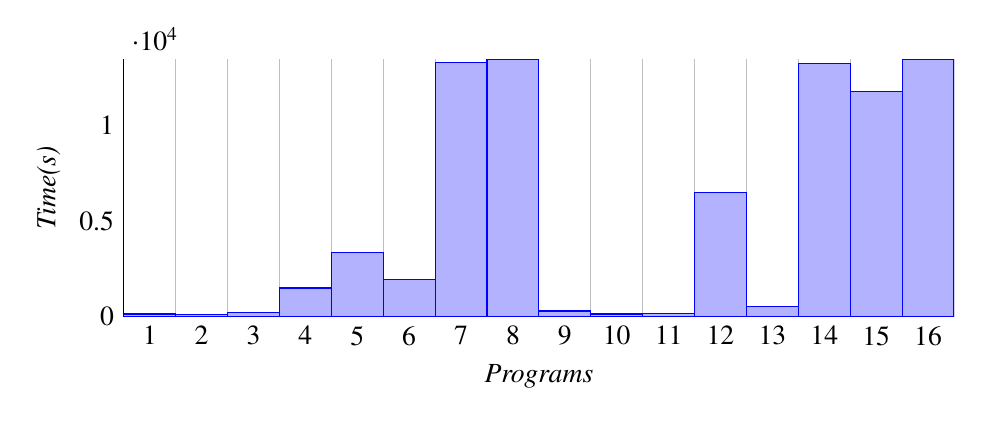
\begin{tikzpicture}
                  \begin{axis}[
                  height = 0.4\textwidth,
                  width = 1\textwidth,
                  ylabel=\emph{Time(s)},
                  xlabel=\emph{Programs},
                  legend style={at={(0.5,-0.2)},cells={align=left},
                  anchor=north,legend columns=1},
                  ybar interval = 1,
                  axis lines=left, % remove top and right axis lines
                  tick align=inside, % move ticks inside the plot area
                  xtick align=inside,
                  axis line style={-}, % remove arrow heads from axes
                  xtick style={draw=none}, % remove ticks
                  ytick style={draw=none},
                  enlarge x limits=false, % don't extend x limits beyond the data range
                  ymajorgrids=false, % remove y grid lines
                  legend style={draw=none}, % remove border from legend
                  ]
                  %Model Ouput
                  \addplot
                  coordinates {
                  (16,13471.964629)
                  (15,11808.325128)
                  (14,13243.207864)
                  (13,551.798543)
                  (12,6483.945198)
                  (11,163.094611)
                  (10,142.0037)
                  (9,300.228418)
                  (8,13449.994491)
                  (7,13328.27705)
                  (6,1969.828764)
                  (5,3351.88337)
                  (4,1500.01275)
                  (3,196.948547)
                  (2,103.677106)
                  (1,139.825496)
                  (0,0)
                  };

                  \end{axis}
            \end{tikzpicture}
      }
      \caption{Waktu Pelatihan Model}
      \label{tb:HasilPengujianTrainTime}
\end{figure}
  

\begin{longtable}{|l|r|r|r|r|r|r|r|}
      \caption{Waktu Generasi Data.}
      \label{tb:HasilPengujianGenTime} \\
      \hline
      \rowcolor[HTML]{C0C0C0}
      \textbf{Program} & \textbf{1\%} & \textbf{2\%} & \textbf{5\%} & \textbf{10\%} & \textbf{25\%} & \textbf{50\%} & \textbf{Per Row Time (s)} \\
      \hline
      Age Analysis & 1 & 2 & 5 & 10 & 24 & 47 & 0.12 \\
      \hline
      Commute Type & 1 & 2 & 3 & 6 & 15 & 30 & 0.14 \\
      \hline
      Commute T-F & 2 & 3 & 7 & 14 & 35 & 69 & 0.45 \\
      \hline
      Customers & 11 & 21 & 53 & 105 & 261 & 522 & 0.05 \\
      \hline
      Delays & 26 & 51 & 126 & 251 & 627 & 1254 & 0.04 \\
      \hline
      Delivery Faults & 16 & 32 & 78 & 156 & 390 & 780 & 0.04 \\
      \hline
      External Call & 100 & 200 & 500 & 1000 & 2500 & 5000 & 0.007 \\
      \hline
      Find Salary & 100 & 200 & 500 & 1000 & 2500 & 4999 & 0.007 \\
      \hline
      Flight Distance & 3 & 5 & 12 & 23 & 57 & 113 & 0.28 \\
      \hline
      Income Agg. & 1 & 2 & 5 & 10 & 25 & 49 & 0.10 \\
      \hline
      Inside Circle & 2 & 3 & 7 & 13 & 32 & 63 & 0.06 \\
      \hline
      Loan Type & 48 & 95 & 238 & 475 & 1187 & 2373 & 0.03 \\
      \hline
      Movie Rating & 5 & 9 & 22 & 44 & 110 & 220 & 0.06 \\
      \hline
      Number Series & 98 & 195 & 487 & 974 & 2434 & 4867 & 0.01 \\
      \hline
      Student Grade & 90 & 179 & 448 & 895 & 2238 & 4475 & 0.01 \\
      \hline
      Word Count & 100 & 200 & 500 & 1000 & 2500 & 5000 & 0.007 \\
      \hline
\end{longtable}

\cleardoublepage

% Bab 5 Kesimpulan dan Saran
\chapter{KESIMPULAN DAN SARAN}
\label{chap:kesimpulandansaran}

% Ubah bagian-bagian berikut dengan isi dari penutup

\section{Kesimpulan}
\label{sec:kesimpulan}

Berdasarkan hasil pengujian yang \lipsum[1][1-3] sebagai berikut:

\begin{enumerate}[nolistsep]

  \item Pembuatan \lipsum[2][1-3]

  \item \lipsum[2][4-6]

  \item \lipsum[2][7-10]

\end{enumerate}

\section{Saran}
\label{chap:saran}

Untuk pengembangan lebih lanjut pada \lipsum[1][1-3] antara lain:

\begin{enumerate}[nolistsep]

  \item Memperbaiki \lipsum[2][1-3]

  \item \lipsum[2][4-6]

  \item \lipsum[2][7-10]

\end{enumerate}

\cleardoublepage

\chapter*{DAFTAR PUSTAKA}
\addcontentsline{toc}{chapter}{DAFTAR PUSTAKA}
\renewcommand\refname{}
\vspace{2ex}
\renewcommand{\bibname}{}
\begingroup
\def\chapter*#1{}
\printbibliography
\endgroup
\cleardoublepage

% Lampiran
\chapter*{LAMPIRAN}\label{chap:lampiran}

% PROGRAM WITH TITIAN
\appendix{Kode \emph{Age Analysis}}
\label{app:ageAnalysis}
\lstinputlisting[
  language=Scala,
  nolol,
]{program/scala/benchmark/ageAnalysis.scala}

\appendix{Kode \emph{Commute Type}}
\label{app:commuteType}
\lstinputlisting[
  language=Scala,
  nolol,
]{program/scala/benchmark/commuteType.scala}

\appendix{Kode \emph{Commute Type Full}}
\label{app:commuteTypeFull}
\lstinputlisting[
  language=Scala,
  nolol,
]{program/scala/benchmark/commuteTypeFull.scala}

\appendix{Kode \emph{Customers}}
\label{app:customers}
\lstinputlisting[
  language=Scala,
  nolol,
]{program/scala/benchmark/customers.scala}

\appendix{Kode \emph{Delays}}
\label{app:delays}
\lstinputlisting[
  language=Scala,
  nolol,
]{program/scala/benchmark/delays.scala}

\appendix{Kode \emph{Delivery Faults}}
\label{app:deliveryFaults}
\lstinputlisting[
  language=Scala,
  nolol,
]{program/scala/benchmark/deliveryFaults.scala}

\appendix{Kode \emph{External Call}}
\label{app:externalCall}
\lstinputlisting[
  language=Scala,
  nolol,
]{program/scala/benchmark/externalCall.scala}

\appendix{Kode \emph{Find Salary}}
\label{app:findSalary}
\lstinputlisting[
  language=Scala,
  nolol,
]{program/scala/benchmark/findSalary.scala}

\appendix{Kode \emph{Flight Distance}}
\label{app:flightDistance}
\lstinputlisting[
  language=Scala,
  nolol,
]{program/scala/benchmark/flightDistance.scala}

\appendix{Kode \emph{Income Aggregation}}
\label{app:incomeAggregation}
\lstinputlisting[
  language=Scala,
  nolol,
]{program/scala/benchmark/incomeAggregation.scala}

\appendix{Kode \emph{Inside Circle}}
\label{app:insideCircle}
\lstinputlisting[
  language=Scala,
  nolol,
]{program/scala/benchmark/insideCircle.scala}

\appendix{Kode \emph{Loan Type}}
\label{app:loanType}
\lstinputlisting[
  language=Scala,
  nolol,
]{program/scala/benchmark/loanType.scala}

\appendix{Kode \emph{Movie Rating}}
\label{app:movieRating}
\lstinputlisting[
  language=Scala,
  nolol,
]{program/scala/benchmark/movieRating.scala}

\appendix{Kode \emph{Number Series}}
\label{app:numberSeries}
\lstinputlisting[
  language=Scala,
  nolol,
]{program/scala/benchmark/numberSeries.scala}

\appendix{Kode \emph{Student Grade}}
\label{app:studentGrade}
\lstinputlisting[
  language=Scala,
  nolol,
]{program/scala/benchmark/studentGrade.scala}

\appendix{Kode \emph{Word Count}}
\label{app:wordCount}
\lstinputlisting[
  language=Scala,
  nolol,
]{program/scala/benchmark/wordCount.scala}

% API WITH FASTAPI
\appendix{Kode FastAPI: \emph{api.py}}
\label{app:api}
\lstinputlisting[
  language=Python,
  nolol,
]{program/python/api.py}

\appendix{Kode FastAPI: \emph{gpt2\_dataset.py}}
\label{app:gpt2Dataset}
\lstinputlisting[
  language=Python,
  nolol,
]{program/python/distilgpt2/gpt2\_dataset.py}

\appendix{Kode FastAPI: \emph{model.py}}
\label{app:model}
\lstinputlisting[
  language=Python,
  nolol,
]{program/python/distilgpt2/model.py}

% API USAGE WITH SCALA
\appendix{Kode Penggunaan API: \emph{main.scala}}
\label{app:main}
\lstinputlisting[
  language=Scala,
  nolol,
]{program/scala/main.scala}
\cleardoublepage


% Biografi penulis
\begin{center}
  \Large
  \textbf{BIOGRAFI PENULIS}
\end{center}

\addcontentsline{toc}{chapter}{BIOGRAFI PENULIS}

\vspace{2ex}

\begin{wrapfigure}{L}{0.3\textwidth}
  \centering
  \vspace{-3ex}
  % Ubah file gambar berikut dengan file foto dari mahasiswa
  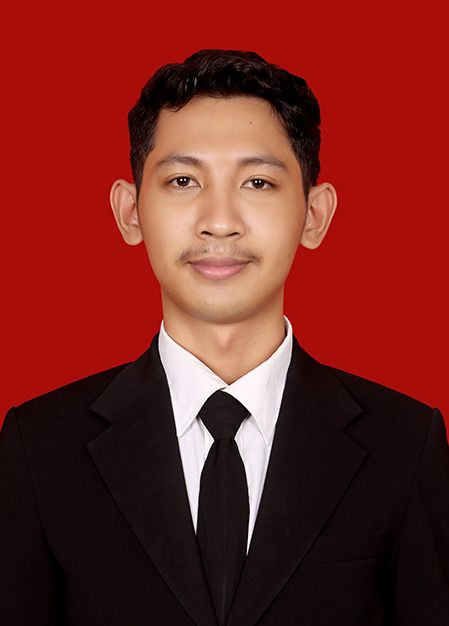
\includegraphics[width=0.3\textwidth]{gambar/jabalnur.jpeg}
  \vspace{-4ex}
\end{wrapfigure}

% Ubah kalimat berikut dengan biografi dari mahasiswa
\name{}, dilahirkan di Pangkep, 29 Juni 2000, merupakan anak pertama dan terakhir
dari kedua orang tuanya. Penulis telah menyelesaikan pendidikan di SDN 14 Bonto Tene, 
SMPN 2 Pangkep, SMAN 11 Pangkep, dan S1 Teknik Informatika Universitas Hasanuddin. Pada
tahun 2020, penulis mengikuti SBMPTN dan diterima di Institut Teknologi Sepuluh Nopember
pada program studi S1 \department{} Fakultas \facultyshort{} \institute{} dengan NRP 5025201241.

Di departemen \department{}, penulis aktif dalam berbagai kegiatan organisasi 
dan kepanitiaan. Penulis sempat menjabat sebagai Wakil Ketua Himpunan Eksternal
Departemen Teknik Informatika pada tahun 2023. Penulis dapat dihubungi melalui 
email \href{mailto:\email}{\email}.


% \cleardoublepage

\end{document}
